\documentclass[12pt]{extarticle}
\usepackage{geometry}
\geometry{
a4paper,
total={170mm,257mm},
left=20mm,
top=20mm,
headheight=12pt
}

%\usepackage[parfill]{parskip} % Activate to begin paragraphs with an empty line rather than an indent
\usepackage{graphicx} % Use pdf, png, jpg, or eps§ with pdflatex; use eps in DVI mode
% TeX will automatically convert eps --> pdf in pdflatex
\usepackage[labelfont=bf]{caption}
\usepackage{float}

\usepackage{amssymb,amsmath,amsthm}
\usepackage{commath}
\usepackage[hyphens]{url}
\usepackage[dvipsnames]{xcolor}
\usepackage[unicode=true,colorlinks=true,urlcolor=CadetBlue,citecolor=black,linkcolor=black]{hyperref}
\PassOptionsToPackage{hyphens}{url} % url is loaded by hyperref
\usepackage{authblk}
\usepackage{longtable}
\usepackage{multirow}
\usepackage{booktabs}
\usepackage{lipsum}  
\usepackage[title,page]{appendix}
\usepackage{chngcntr}
%\usepackage{end float}
 \usepackage{subcaption}
 \usepackage{cleveref}

%SetFonts
% newtxtext+newtxmath
\usepackage{newtxtext} %loads helv for ss, txtt for tt
\usepackage{amsmath}
\usepackage[bigdelims]{newtxmath}
\usepackage[T1]{fontenc}
\usepackage{textcomp}
%SetFonts

% less space before sections 
% https://tex.stackexchange.com/a/101126
%\usepackage{titlesec}
%\titlespacing*{\section}{0pt}{0.5\baselineskip}{0\baselineskip}
%\titlespacing*{\subsection}{0pt}{0.5\baselineskip}{0\baselineskip}
    
% Species names
%% Meta-Command for defining new species macros
\usepackage{xspace}

\allowdisplaybreaks

\newcommand{\species}[3]{%
  \newcommand{#1}{\gdef#1{\textit{#3}\xspace}\textit{#2}\xspace}}
  \species{\yeast}{Saccharomyces cerevisiae}{S.~cerevisiae}

% line numbers
\usepackage[displaymath, mathlines]{lineno}
\renewcommand\linenumberfont{\normalfont\small\sffamily}
%\linenumbers
\modulolinenumbers[2]

% Yoav & Lee commands
\newcommand*{\tr}{^\intercal}
\let\vec\mathbf
\newcommand{\matrx}[1]{{\Big[ \stackrel{}{#1}\Big]}}
\newcommand{\diag}[1]{\mbox{diag}\matrx{#1}}
\newcommand{\goesto}{\rightarrow}
\newcommand{\dspfrac}[2]{\frac{\displaystyle #1}{\displaystyle #2} }
\newtheorem{theorem}{Theorem}
\newtheorem{corollary}{Corollary}
\newtheorem{lemma}{Lemma}
\newtheorem{remark}{Remark}
\newtheorem{result}{Result}
\renewcommand\qedsymbol{} % no square at end of proof
\newcommand{\cl}{\mathbf{L}}
\newcommand{\cj}{\mathbf{J}}
\newcommand{\ci}{\mathbf{I}}
\newcommand{\E}{\mathbf{E}}
\DeclareMathOperator{\sign}{sign}
\renewcommand{\d}[1]{\ensuremath{\operatorname{d}\!{#1}}}

% Remus commands
\newcommand{\x}{{\bf x}}
\renewcommand{\d}{{\rm d}}
\newcommand{\e}{{\rm e}}
\newcommand{\erfc}{{\rm erfc}}
\newcommand{\ii}{{\rm i}}

\newcommand{\tmi}{\tau_0\wedge\tau}
\newcommand{\tma}{\tau_0\vee\tau}
\newcommand{\taua}{\tau_{\rm A}}

% Daniel commands

\newcommand{\daniel}[1]{\textcolor{blue}{#1}}
\newcommand{\presc}{p_\text{rescue}}
\newcommand{\psgv}{p_\text{SGV}}

% Supplementary
% https://support.authorea.com/en-us/article/how-to-create-an-appendix-section-or-supplementary-information-1g25i5a/
\newcommand{\beginsupplement}{%
      	\setcounter{table}{0}
        \renewcommand{\thetable}{S\arabic{table}}%
        \setcounter{figure}{0}
        \renewcommand{\thefigure}{S\arabic{figure}}%
		\setcounter{equation}{0}
        \renewcommand{\theequation}{A\arabic{equation}}%
}

% autoref
\def\equationautorefname{Eq.}

% NatBib
\usepackage[comma,sort]{natbib}

%%%%%%%%%%%%%%%%%%%%%%%%%%%%%%%%%%%%%%%%%%%%%%%%%%%%%%

% Title page
\title{The role of aneuploidy in the evolution of cancer drug resistance}
% Authors
\renewcommand\Affilfont{\small}

\author[1]{Remus Stana}
\author[2]{Uri Ben-David}
\author[3]{Daniel B. Weissman}
\author[1,*]{Yoav Ram}
\affil[1]{School of Zoology, Faculty of Life Sciences, Tel Aviv University, Tel Aviv, Israel}
\affil[2]{Department of Human Molecular Genetics and Biochemistry, Faculty of Medicine, Tel Aviv University, Tel Aviv, Israel}
\affil[3]{Department of Physics, Emory University, Atlanta, GA}
\affil[*]{Corresponding author: yoav@yoavram.com}
 
%%%%%%%%%%%%%%%%%%%%%%%%%%%%%%%%%%%%%%%%%%
\begin{document}
\maketitle

% MESSAGES ok
% 1. aneuploidy increases the prob of rescue -- reduces the tumor threshold size for rescue
% 2. aneuploidy changes the survival curve in a distinct way

% FIGURES ok
% Fig 1A: model graph chart
% Fig 1B: Delta_w, Delta_a, Delta_m illustration

% Fig 2: example simulations - w_t, a_t, m_t over time 
% 	A u=0; B Delta_a << 0; C Delta_a ~ 0; D Delta_a >>0  

% Fig 3A: prob rescue vs N for various Delta_a; markup N*
% Fig 3B: N* vs Delta_a
% Fig 3C: N* vs u/v

% Fig 4: survival curves
% 	A u=0; B Delta_a << 0; C Delta_a ~ 0; D Delta_a >>0

%%%%%%%%%%%%%%%%%%%%%%%%%%%%%%%%%%%%%%%%%%
\begin{abstract}
Evolutionary rescue is the process by which a population survives a sudden environmental change that initially causes the population to decline towards extinction.
A prime example of evolutionary rescue is the ability of cancer to survive exposure to various treatments. 
One evolutionary mechanism by which a population of cancer cells can to adapt to chemotherapy is aneuploidy. 
Aneuploid cancer cells can have higher fitness in an environment altered by anti-cancer drugs, e.g., because of incomplete pathways targeted by the drugs. 
Indeed, aneuploidy is highly prevalent in tumors, and moreover, some anti-cancer drugs fight cancer by increasing chromosomal instability.
Here, we examine how aneuploidy impacts the fate of a population of cancer cells. We use multi-type branching processes to approximate the probability that a tumor survives drug treatment as a function of the initial tumor size, and rates at which aneuploidy and other beneficial mutations occur, and the growth rates of the sensitive and resistant cells. Additionally, we investigate what effect having a fraction of tumor cells being aneuploid before the onset of therapy have on the probability of evolutionary rescue.  We also approximate the mean recurrence time for the tumor to revert back to its initial size.
We find that aneuploidy can play an important role in the relapse of secondary tumors who have not yet been detected and thus are smaller in size.
% TODO missing something here... ok
\end{abstract}

Keywords: whole-chromosome duplication, evolutionary model, adaptive evolution, cancer, drug resistance, chromosome instability

\newpage
%%%%%%%%%%%%%%%%%%%%%%%%%%%%%%%%%%%%%%
\section*{Introduction}

%%%%%%

\paragraph{Aneuploidy in cancer.}  Each year approximately 10 million people die from cancer \citep{kocarnik2022cancer}, so understanding the factors that contribute to failure of interventions is of great importance. One hypothesized factor is aneuploidy, where cells are characterized by an imbalanced karyotype and chromosome copy number alterations \citep{schukken2018cin}, caused by chromosomal instability, the mitotic process in which cells suffer from chromosome mis-segregation that leads to aneuploidy. Importantly, aberrations in chromosome copy number have been shown to allow cancer cells to survive under stressful conditions such as drug therapy \citep{lukow2021chromosomal,rutledge2016selective}. Indeed, cancer cells are often likely to be aneuploid, and aneuploidy is associated with poor patient outcomes \citep{ben2020context,smith2018systematic}. 

 \citet{ippolito2021gene} induced aneuploidy in cancer cell lines by exposing them to reversine, a small-molecule inhibitor of the mitotic kinase Mpsi1, and then to chemotherapeutic agents such as vemurafenib. Reversine-treated cells had higher proliferation rate in the environment altered by anti-cancer drugs compared to wildtype cancer cells.
 Similarly, \citet{lukow2021chromosomal} induced aneuploidy in cancer cells and observed that such cells have an advantage compared to wildtype cells during chemotherapy, despite having lower fitness before the onset of chemotherapy.
One proposed mechanism through which aneuploidy is able to confer resistance to chemotherapeutics is by antagonizing cell division, which prevents the drugs from damaging DNA and microtubules \citep{replogle2020aneuploidy}.
 
An important aspect of aneuploidy is the rate with which cells become aneuploid, which is several orders of magnitude higher than the beneficial mutation rate \citep{bakker2023predicting}. Consequently, a cell exposed to a stress such as chemotherapeutic drugs can acquire aneuploidy faster when compared to acquiring a mutation, especially when several proposed anti-cancer drugs elevate the rate of mis-segregation in order to fight cancer \citep{lee2016effects}.

\paragraph{Evolutionary rescue.} Populations adapted to a certain environment are vulnerable to environmental changes, which might cause extinction of the population. Examples of such environmental changes include climate change, invasive species or the onset of drug therapies. Adaptation is a race against time as the population size decreases in the new environment~\citep{tanaka2022surviving}. 
\emph{Evolutionary rescue} is the process where the population acquires a trait that increases fitness in the new environment such that extinction is averted. It is mathematically equivalent to the problem of crossing of fitness valley \citep{weissman2009rate,weissman2010rate}.
There are three potential ways for a population to survive environmental change: migration to a new habitat similar to the one before the onset of environmental change \citep{harsch2014keeping,cobbold2020should,zhou2022range}; adaptation by phenotypic plasticity without genetic modification \citep{carja2019evolutionary,carja2017evolutionary,levien2021non,gunnarsson2020understanding}; and adaptation through genetic modifications, e.g., mutation \citep{gomulkiewicz1995does,uecker2014evolutionary,uecker2016role,uecker2011fixation,orr2014population}.

\citet{gunnarsson2020understanding} analyze a model where a tumor consisting of two populations of cancer cells, one drug resistant and the other drug sensitive, is able to evade extinction by cells switching between the two phenotypes through epigenetic mutations. They found that even when the drug resistant type is barely viable the epimutations have the effect of guaranteeing evolutionary rescue. Evolutionary rescue in one step in which an initially declining population, after a sudden environmental change, has to acquire a mutation has been studied in the context of population genetics  by \citep{orr2008population,orr2014population}. They analyzed a model where the mutant strain is present in small number at the onset of therapy and concluded that this can significantly enhance the chance that the population will survive. 

Most models focus on the probability that at least one mutation rescues the population. How multiple mutations contribute to the survival of the population is less explored, but \citet{wilson2017soft} have shown that evolutionary rescue is significantly enhanced by soft selective sweeps when multiple mutations contribute.  Evolutionary rescue that requires two successive mutations has been investigated using diffusion approximation by \citet{martin2013probability}.

Here we build on previous work on evolutionary rescue after a sudden environment change caused by the initiation of chemotherapy. We wish to understand what effect does aneuploidy have on the probability of evolutionary rescue when it acts as an intermediary between the wildtype and the mutant cancer cells. We also calculate the mean time that an initially declining tumor cell population reaches its pre-treatment size. Given that aneuploidy is present in many tumors even before the onset of therapy \citep{lukow2021chromosomal} we also take into consideration the effect that standing genetic variation has on the tumor dynamics. Additionally, we are interested in the timescale of evolutionary rescue and the effect that aneuploidy has on the time necessary for the tumor to overcome drug therapy.

%%%%%%%%%%%%%%%%%%%%%%%%%%%%%%%%%%%%%%%%%%
\section*{Methods}

\paragraph{Evolutionary model.}
We follow the number of cancer cells that have one of three different genotypes at time $t$: wildtype, $w_t$; aneuploid, $a_t$; and mutant, $m_t$. 
These cells divide and die with rates $\lambda_k$ and $\mu_k$ (for $k=w, a, m$).
The difference between the division and death rate is $\Delta_k = \lambda_k-\mu_k$.
We assume the population of cells is under a strong stress, such as drug therapy, to which the wildtype genotype is susceptible or sensitive and therefore $\Delta_w<0$, whereas the mutant is resistant to the stress, $\Delta_m>0$.
We analyze three scenarios: in the first, aneuploid cells are partially resistant, $\Delta_m>\Delta_a>0$; in the second, aneuploid cells are tolerant, $0>\Delta_a>\Delta_w$ \citep[see][for the distinction between susceptible, resistant, and tolerant]{brauner2016distinguishing}; in the third, aneuploid cells are non-growing, stationary or growing or dying only very slowly, that is, either slightly tolerant or slightly resistant, such that $\Delta_a \approx 0$, in a sense that we will make precise below. 
We assume that both chromosomal missegregation and mutation occur during the process of mitosis. 
Wildtype cells may divide and then missegregate to become aneuploids at rate $u\lambda_w$. Both aneuploid and wildtype cells may divide and mutate to become mutants at rates $v\lambda_{a}$ and $v\lambda_{w}$, respectively.
To model standing genetic variation, we assume that before the onset of therapy, wildtype cells become aneuploid with rate $\tilde{u}\lambda_w$ (which may differ from $u \lambda_w$) and that aneuploidy confers a fitness cost $s$ in the drug-free environment, that is, we assume that aneuploid cells have an increased death rate compared to wildtype cells in a drug-free environment.
See \Cref{figureAneuploidy} for a schematic representation of the model and \Cref{sampleTrajectories} for sample trajectories of the different genotypes. 

%%%%%%%%%%%%%%%%%%%%%%%%%%%%%%%%%%%%%%%%

\paragraph{Stochastic simulations.} 
Simulations are performed using the \emph{Gillespie stochastic simulation algorithm} \citep{gillespie1976general,gillespie1977exact} implemented in Python \citep{python}.
The simulation monitors the number of cells of each type: wildtype, aneuploid, and mutant. 
The wildtype population initially consists of $w_0=N$ cells, whereas the other cell types are initially absent.

The state of the stochastic system at time $t$ is represented by the triplet $\left(w_t,a_t,m_t\right)$. The following describes the events that may occur (right column), the rates at which they occur (middle column), and the effect these events have on the state (left column, see \Cref{figureAneuploidy}):

\begin{subequations}
\begin{flalign*}
(+1,0,0)&:\quad \lambda_ww_t\left(1-u-v\right)\quad\left(\text{birth of wildtype cell}\right),\\
(-1,0,0)&:\quad \mu_ww_t\quad\left(\text{death of wildtype cell}\right),\\
(0,+1,0)&:\quad u\lambda_ww_t\quad\left(\text{wildtype cell divides and becomes aneuploid}\right),\\
(0,0,+1)&:\quad v\lambda_ww_t\quad\left(\text{wildtype cell divides and becomes mutant}\right),\\
(0,+1,0)&:\quad \lambda_aa_t\left(1-v\right)\quad\left(\text{birth of aneuploid cell}\right),\\
(0,-1,0)&:\quad \mu_aa_t\quad\left(\text{death of aneuploid cell}\right),\\
(0,0,+1)&:\quad v\lambda_aa_t\quad\left(\text{aneuploid cell divides and becomes mutant}\right),\\
(0,0,+1)&:\quad \lambda_mm_t\quad\left(\text{birth of mutant cell}\right),\\
(0,0,-1)&:\quad \mu_mm_t\quad\left(\text{death of mutant cell}\right).
\end{flalign*}
\end{subequations}
For the remaining of this paper we assume that the division rates for wildtype and aneuploid cells can be written as $\lambda_ww_t\left(1-u-v\right)\approx \lambda_ww_t$ and $\lambda_aa_t\left(1-v\right)\approx\lambda_aa_t$ because $u,v\ll1$ (see Table \ref{table1}).
Each iteration of the simulation loop starts with computing the rates $\nu_k$ of each event $k$.
We then draw the time until the next event, $\Delta t$, from an exponential distribution whose rate parameter is the sum of the rates of all events, such that $\Delta t \sim \text{Exp}(\sum_j \nu_j)$.
Then, we randomly determine which event occurred, where the probability for event $k$ is $p_k = \nu_k/\sum_j \nu_j$.
Finally, we update the number of cells of each type according to the event that occurred and update the time from $t$ to $t+\Delta t$.
We repeat these iterations until either the population becomes extinct (the number of cells of all types is zero) or the number of mutant cells is high enough so that its extinction probability is $<0.1\%$, that is until
\begin{equation*}
m_t > \left\lfloor\frac{3\log{10}}{\log{\left(\lambda_m / \mu_m\right)}}\right\rfloor + 1 ,
\end{equation*}
which we obtain by solving $1-(1-p_m)^{m_t}=0.999$ for $m_t$ with $p_m=\Delta_m/\lambda_m$ as the probability that a single mutant escapes stochastic extinction  (see Appendix A).

When simulations are slow (e.g., due to large population size), we use $\tau$-leaping \citep{gillespie2001approximate}, where we assume that the change in the number of cells of genotype $k$ in a fixed time interval $\Delta t$ is Poisson distributed with mean $\nu_k \Delta t$. If the change in the number of cells is negative and larger than the subpopulation size then the subpopulation size is updated to be zero. 

%%%%%%%%%%%%%%%%%%%%%%%%%%%%%%%%%%%%%%%%
% YR:  I commented this out because it is entirely standard
%\paragraph{Bootstrapping}
%We  use bootstrap resampling method in order to compute  confidence intervals for the mean threshold tumor sizes and mean times by resampling 100 times with replacement from the data set obtained from simulations. We then compute the interval which contain $95\%$ of the means of each resampled set.

%%%%%%%%%%%%%%%%%%%%%%%%%%%%%%%%%%%%%%%%

\paragraph{Parameterization.}
To parametrize the simulations, we assume that the cells under consideration are melanoma cells and rely on \citet{rew2000cell} and \citet{bozic2013evolutionary} for the division and death rates, respectively. 
\citet{rew2000cell} report \emph{in vivo} measurements of the potential doubling times (the waiting time for the number of cells in the tumor to double disregarding cell death) for a large set of cancer types. The division rate is obtained as $\lambda=\log{2} / T \approx 0.1$ per day. We select this to be the division rate for wildtype and mutant cells. %We select the mutant death rate $\mu_m=0.09\text{ days}^{-1}$ such that $\Delta_m>0$.

\citet{bozic2013evolutionary} report the growth rate $\Delta_w$ for wildtype melanoma cancer cells from which they deduce the death rate $0.11 \le \mu_w \le 0.17$. We use  $\mu_w=0.14$ per day. Additionally, they observe the growth rate of cancer cells prior to treatment to be 0.01, which we use as the growth rate of mutant cells, which are resistant to the drug. Thus, we use $\mu_m=0.1-0.01=0.09$ per day as the death rate for mutant cells.

 Aneuploid death rate $\mu_a$ is set to the same value as the mutant death rates, $\mu_m=0.09$ per day, given that aneuploidy increases resistance to the drug, such as cisplatin, by antagonizing cell division \citep{replogle2020aneuploidy}. Aneuploid division rate is selected such that the aneuploid growth rate $\Delta_w\ll\Delta_a\ll\Delta_m$ which means that $0.06 \le \lambda_a \le 0.1$. For most of our simulations we use $\lambda_a=0.0899$ per day, such that aneuploidy can only act as a \emph{stepping stone} for the generation of the mutant that rescues the cancer cell population.

We assume the mutation rate is $10^{-7}$ per gene per cell division \citep{loeb2001mutator} and since we assume that a single target gene confers resistance to the drug, we use $v=10^{-7}$ per cell division. 
\citet{bakker2023predicting} determined that the missegregation rate must be between $10^{-3}-10^{-2}$ per chromosome per cell division with the optimal value being $6.21\times10^{-3}$ per chromosome per cell division. \citet{ippolito2021gene} observed that trisomy in Chr II and VI are most likely to confer increased resistance against the chemotherapeutic agent vemurafenib for A375 cells. We assume that if a tumor is aneuploid then it most likely has trisomy \citep{gisselsson2010generation} in the pre-treatment environment and that cells with more than one trisomy are very unlikely to survive. Additionally, we assume that all trisomies are equally likely and, as a result, we select $u=10^{-2}$ per cell division. For the missegregation rate in the drug-free environment, $\tilde{u}$, we use the lower-end value of $\tilde{u}=2\times10^{-3}$ per cell division, as some drugs increase the rate of aneuploidy~\citep{wang2019molecular,mason2017functional}.

The fitness cost $s$ of aneuploidy before the onset of therapy is difficult to estimate as we are interested in a specific type of aneuploidy which improves the fitness of cancer cells in an environment altered by drugs.
We derive $s$ by using the formula $s=\tilde{u}\lambda_w / f$, where $f$ is the fraction of aneuploid cancer cells. To estimate $f$, we note that \citet{lukow2021chromosomal} mixed together wildtype and aneuploid A375 melanoma cells at $50:50$ ratio, cultured them in drug-free environment and observed the ratio evolve as a function of time with the aneuploid cells declining to $15\%$ after 24 days. We obtain the fitness cost $s$ using the formula $s=\abs{\log\left[0.15/(1-0.15)\right]/24}\approx0.07$ per day \citep{chevin2011measuring}. As a result, the fraction of cancer cells with ``beneficial'' aneuploidy is $f=2\times10^{-3}\times10^{-1}/0.07=0.284\%$ (i.e. $0.284\%$ of pre-treatment cancer cells have the ``beneficial'' aneuploidy).


We note that when we refer to wildtype cancer cells we include those cells that have any aneuploidy except trisomy in Chr II and VI as those are the aneuploid cells which are hypothesized to have higher fitness in the environment altered by drugs such as vemurafenib.
%%%%%%%%%%%%%%%%%%%%%%%%%%%%%%%%%%%%%%%%

\paragraph{Density-dependent growth.}

In our analytical calculations, we assume that lineages produced by cells from the initial population divide and die independently of each other.
Of course, the cells will actually compete for resources, but we expect that this can be neglected because the drug will
cause the cell density to rapidly drop far below the carrying capacity at which these interactions are important.
To test this, we simulate a logistic growth model, with division and death rates given by:
\begin{align*}
\lambda_w' &= \lambda_w , \\
\mu_w' &= \mu_w ,\\
\lambda_a' &= \lambda_a ,\\ 
\mu_a' &= \mu_a + \lambda_a\frac{w+a+m}{K} ,\\
\lambda_m' &= \lambda_m ,\\ 
\mu_m' &= \mu_m + \lambda_m\frac{w+a+m}{K} ,
\end{align*}
where $K$ is the tumor carrying capacity. 
The effective carrying capacity of this model is $K_e=K\Delta_a/\lambda_a\approx10^6$ for $K=10^8, \lambda_a=0.0901,\mu_a=0.09$, where we define the effective carrying capacity to be the population size at which the aneuploid division rate is equal to the aneuploid death rate. 

%%%%%%%%%%%%%%%%%%%%%%%%%%%%%%%%%%%%%%%%

\paragraph{Code and data availability.} All source code is available online at~\url{https://github.com/yoavram-lab/EvolutionaryRescue}.

%%%%%%%%%%%%%%%%%%%%%%%%%%%%%%%%%%%%%%%%

\section*{Results}


%%%%%%%%%%%%%%%%%%%%%%%%%%%%%%%%%%%%%
\subsection*{Evolutionary rescue probability}

In our model, \emph{evolutionary rescue} occurs when resistant cells appear and establish (avoid random extinction) in the population  ($m_t \gg 1$) before the population becomes extinct ($w_t=a_t=m_t=0$).
Aneuploidy may contribute to evolutionary rescue by either preventing (when $\Delta_a>0$) or delaying (when $0>\Delta_a>\Delta_w$) the extinction of the population before mutant cells appear and establish.
We assume independence between clonal lineages starting from an initial population of $N$ wildtype cells (we check the effect of density-dependent growth on our results below).
We therefore define $p_w$ as the probability that a lineage starting from a single wildtype cell avoids extinction by acquiring drug resistance.
Thus, $N^*=1/p_w$ is the threshold tumor size above which evolutionary rescue is very likely, and the rescue probability is given by 
\begin{equation} \label{eq:rescue_prob} 
\presc = 
1-\left(1-p_w\right)^N \approx
1-\e^{-Np_w} = 
1-e^{-N/N^*} ,
\end{equation}
where the approximation $(1-p_w)\approx e^{-p_w}$ assumes that $p_w$ (but not necessarily $N p_w$) is small.
Indeed, when $N<1/p_w$, then the probability for evolutionary rescue is $\presc \approx N p_w$  and when $N > 1/p_w$, it is $\presc \approx 1$, justifying the definition of $N^*$ as the threshold tumor size for evolutionary rescue. 

We use the theory of multi-type branching processes to find approximate expressions \cref{eq:pw_parttolerant,eq:pw_partrest,eq:pw_tolerant} for $p_w$ in different regimes (see appendix~\ref{sec:appendix-surv-prob}). 
Substituting these into $N^*=1/p_w$, we find approximations for the threshold tumor size, $N^*$. 
For these approximations, an important quantity is $T^* = (4 v \lambda_a^2 \Delta_m/\lambda_m)^{-1/2}$, which is the critical time an aneuploid lineage needs to survive to produce a resistant mutant that avoids random extinction.
First, if aneuploidy is very rare ($u\lambda_a T^*< 1$), or if aneuploidy is rare ($u\lambda_a < -\Delta_a$) and very sensitive to the drug ($\Delta_a T^* < -1$), then evolutionary rescue will likely occur by a direct resistance mutation in a sensitive wildtype cell without the involvement of aneuploidy, such that 
\begin{equation} \label{eq:N_m}
N_m^* \approx \frac{\abs{\Delta_w}}{v\lambda_w}  \frac{\lambda_m}{\Delta_m} .
\end{equation}
Here, $\abs{\Delta_w}/\left(v\lambda_w\right)$ is the ratio of the rate at which wildtype cells are decreasing in number and the rate at which they are mutating. Notably, the aneuploidy parameters ($u$, $\lambda_a$, $\mu_a$) do not affect $N_m^*$.

Otherwise, aneuploidy is frequent enough ($u\lambda_a > \max{\left(-\Delta_a, 1/T^*\right)}$) to affect the evolution of drug resistance. 
The threshold tumor size can then be approximated by one of the following cases, depending on $\Delta_a T^*$, the change in the aneuploid log-population size during the critical time,
\begin{equation}  \label{eq:N_a}
\begin{aligned}
N_a^* \approx 
  \frac{\abs{\Delta_w}}{u\lambda_w} \cdot \begin{cases}
    \frac{\abs{\Delta_a}}{v\lambda_a}  \frac{\lambda_m}{\Delta_m} ,&
  \Delta_a T^* \ll -1 \text{ (tolerant aneuploids)},\\ 
  %\left(\frac{\lambda_a}{v}  \frac{\lambda_m}{\Delta_m}\right)^{1/2} ,&
  2\lambda_a T^* ,&
  -1 \ll \Delta_a T^* \ll 1  \text{ (stationary aneuploids)},\\ 
  \frac{\lambda_a}{\Delta_a} ,&
   \Delta_a T^* \gg 1 \text{ (resistant aneuploids)}.
  \end{cases}
\end{aligned}
\end{equation}
These approximations perform very well when compared to results of stochastic evolutionary simulations (\Cref{rescue_prob,rescue_threshold}).
The first line describes the case in which aneuploid cells are still effectively killed by the treatment, but not as quickly as the wild type. 
In the second case, aneuploid cells are sufficiently resistant that the expected size of each aneuploid lineage is roughly 1.
In both of these cases, aneuploidy increases the probability of rescue by slowing or halting the decrease of the cancer population, allowing more opportunities for producing resistant mutants. 
In the third case, aneuploid cells are sufficiently resistance for the cancer population to re-grow the tumor even without additional resistance mutations.
Notably, in this case the mutant parameters ($v$, $\lambda_m$, and $\Delta_m$) do not affect $N_a^*$ beyond their effect on $T^*$.
In all cases, $N_a^*$ is proportional to $1/u$ such that increasing the missegregation rate $u$ will decrease the threshold tumor size (\Cref{rescue_threshold}B).
Furthermore, increasing the aneuploid growth rate $\Delta_a$ (which appears both in the terms and in the conditions), also reduces the threshold tumor size, with a sharp decrease around $\Delta_a=0$, but the effect is minor when $|\Delta_a|$ is small compared to $T^*$ as this would result in the second case where  $dN_a^*/d\Delta_a=0$ (\Cref{rescue_threshold}A). % TODO these are pretty straightforward - can you glean something more interesting from eq 4? I am still looking for more interesting results from eq4 

Using \cref{eq:N_a,eq:N_m}, we can find the ratio of threshold tumor size for rescue via aneuploidy ($u$ is high) or via direct mutation ($u$ is low),
\begin{equation} \label{eq:N_ratio}
\frac{N^*_a}{N^*_m} \approx \begin{cases}
    \frac{\abs{\Delta_a}}{u\lambda_a} ,&
  \Delta_a T^* \ll -1 ,\\ 
  \frac{1}{u}\left(v  \frac{\Delta_m}{\lambda_m}\right)^{1/2} ,&
  -1 \ll \Delta_a T^* \ll 1  ,\\ 
  v \frac{\Delta_m}{\lambda_m}  \left(u\frac{\Delta_a}{\lambda_a}\right)^{-1}  ,&
   \Delta_a T^* \gg 1 .
  \end{cases}
\end{equation}
As expected, this ratio increases with the mutation rate $v$ and decreases with the aneuploidy rate $u$.
In the first case, $\abs{\Delta_a}/\left(u\lambda_a\right)$ is  the ratio of the expected time for an aneuploid lineage to appear, $1/\left(u\lambda_a\right)$, and the expected time until that lineage disappears, $1/\abs{\Delta_a}$.
In the third case, $\left(v \frac{\Delta_m}{\lambda_m}\right) / \left(u \frac{\Delta_a}{\lambda_a}\right)$ is the ratio of the rates of formation of resistant mutants that avoid extinction and partially resistant aneuploids that avoid extinction.
In the second case, $\frac{1}{u}\left(v  \frac{\Delta_m}{\lambda_m}\right)^{1/2}=\sqrt{\frac{\Delta_a}{u\lambda_a}  v \frac{\Delta_m}{\lambda_m}  \left(u\frac{\Delta_a}{\lambda_a}\right)^{-1}}$, which is the geometric mean of the first and third cases.

Interestingly, increasing both the aneuploid division rate, $\lambda_a$, and the aneuploid death rate, $\mu_a$, such that the growth rate $\Delta_a$ remains constant, leads to decreases in $T^*$, pushing the system to the second case. In this case, increasing the division rate $\lambda_a$ should also increase the mutation rate $v\lambda_a$ in aneuploid cells, as mutations mostly occur during division, so overall the threshold tumor size $N_a^*$ is unaffected by the division rate $\lambda_a$ (i.e., $d \lambda_a T^*/d\lambda_a = 0$). Thus, if aneuploid cells rapidly die due to the drug but compensate by rapidly dividing, further increasing  the division rate will \emph{not} facilitate adaptation.
This is consistent with experimental findings where aneuploidy confers resistance by decreasing the division rate~\citep{replogle2020aneuploidy}.

We can categorize tumors by their size: small tumors with size $N<N_a^*$ that are unlikely to survive treatment, intermediate tumors with size $N_a^* < N < N_m^*$ that rely on aneuploidy for evolutionary rescue, and large tumors with size $N > N_m^*$ that could overcome the effect of drug treatment even without aneuploidy.
For the parameter values in \Cref{table1} with $\lambda_a=0.0899,\mu_w=0.14, u=10^{-2}, v=10^{-7}$, we are in the tolerant aneuploid case, and substituting in \cref{eq:N_a,eq:N_m}, we have $N_a^* \approx 4 \times 10^6$ and $N_m^* \approx 4 \times 10^7$.
Hence, we obtain the ratio $N^*_a/N^*_m \approx 0.11$ (\cref{eq:N_ratio}), that is, aneuploidy reduces the threshold tumor size by approximately 89\%.
Interestingly, the threshold between small and intermediate tumors, $N_a^*$, is similar to the tumor detection threshold of $4 \times 10^6$ cells for a wide variety of tumors as reported by \citet{avanzini2019cancer}.

%%%%%%%%%%%%%%%%%%%%%%%%%%%%%%%%%%%%%%%%%%%%%%%%%%%%%%%%%%%%
\paragraph*{Density-dependent growth.}

In our analysis we used branching processes, which assume that growth (division and death) is density-independent. However, growth may be limited by resources (oxygen, nutrients, etc.) and therefore depend on cell density. 
We therefore performed stochastic simulations of a logistic growth model with a carrying capacity (see Methods). 
We find that our density-independent approximations agree with results of simulations with density-dependent growth for biologically relevant parameter values (\Cref{LogisticPlot}).

%%%%%%%%%%%%%%%%%%%%%%%%%%%%%%%%%%%%%%%%%%%%%%%%%%%%%%%%%%%%
\paragraph*{Standing vs. de-novo genetic variation.}

In the above we assumed that at the onset of drug treatment, the initial tumor consisted entirely of wildtype cells that are drug sensitive.
However, aneuploidy is likely produced even before onset of treatment at some rate $\tilde{u}$ and confers a deleterious fitness effect $s$ in the absence of the drug \citep{replogle2020aneuploidy,giam2015aneuploidy}. Furthermore, the aneuploidy rate in the presence of drugs is likely higher than in their absence, $\tilde{u} < u$ \citep{wang2019molecular,mason2017functional}.
But if the number of cells in the tumor $N$ is large (as expected if the tumor is treated with a drug), there may already be a fraction $f \approx \tilde{u}\lambda_w/s$ of aneuploid cells in the population (here we assume that the drug affects the wildtype death rate but no the division rate and therefore use $\lambda_w$ for the wildtype division rate in the drug-free environment).

Therefore, the threshold tumor size with standing generation variation, $\tilde{N}^*_{a}$, is similar to the threshold with de-novo variation, $N^*_a$, except that the sensitive growth rate $\abs{\Delta_w}$ is replaced with the aneuploidy cost $s$, such that
\begin{equation}\label{eq:Nsgv}
\frac{\tilde{N}^*_{a}}{N^*_{a}} = \frac{u}{\tilde{u}} \; \frac{s}{\abs{\Delta_w}}.
\end{equation}
Comparing this approximation of $\tilde{N}^*_{a}/N^*_{a}$ to results of stochastic simulations, we find that the approximations perform very well (\Cref{rescue_denovo}). 
Standing genetic variation will drive evolutionary rescue if wildtype growth rate $\Delta_w$ is very negative due to a strong effect of the drug on sensitive cells, or if the aneuploidy cost in the drug-free environment, $s$, is small.  
In contrast, de-novo aneuploid cells will have a greater contribution to rescue if the aneuploidy cost $s$ is large, the effect of the drug on sensitive cells is weak ($\Delta_w$ is close to zero), or if the drug induces the appearance of aneuploid cells ($u > \tilde u$).
For example, with  $\lambda_w=0.1,\mu_w=0.14, u=10^{-2}, \tilde{u}=2\times10^{-3}, s=0.07$, the ratio of the threshold tumor sizes for standing vs de-novo variation is $\tilde{N}^*_a/N^*_a \approx 8.75$, which means that de-novo genetic variation is  the main driver of evolutionary rescue.

Using \cref{eq:N_a,eq:N_m,eq:Nsgv}, we can find the ratio of threshold tumor size for rescue via standing genetic variation  to the threshold for rescue via direct mutation,
\begin{equation} \label{eq:N_sgv_ratio}
\frac{\tilde{N}^*_a}{N^*_m}=\frac{\tilde{N}^*_{a}}{N^*_{a}} \frac{N^*_a}{N^*_m} \approx \frac{s}{\abs{\Delta_w}}\begin{cases}
    \frac{\abs{\Delta_a}}{\tilde{u}\lambda_a} ,&
  \Delta_a T^* \ll -1 ,\\ 
  \frac{1}{\tilde{u}}\left(v \frac{\Delta_m}{\lambda_m}\right)^{1/2} ,&
  -1 \ll \Delta_a T^* \ll 1  ,\\ 
  v \frac{\Delta_m}{\lambda_m} \left(\tilde{u}\frac{\Delta_a}{\lambda_a}\right)^{-1}  ,&
   \Delta_a T^* \gg 1 .
  \end{cases}
\end{equation}
Evolutionary rescue through direct mutation is more likely if the cost of aneuploidy $s$ is very large or the effect of the drug $\Delta_w$ is small.  In contrast, standing genetic variation will drive adaptation if the pre-treatment chromosome missegreagation rate $\tilde{u}$ is very large. The ratio does not depend on the rate of chromosome missegregation induced by the drug $u$. However, if the aneuploid growth rate $\Delta_a$ increases, then evolutionary rescue is driven by standing genetic variation. For the parameter values of  $\lambda_w=0.1, \lambda_a=0.0899,\lambda_m=0.1,\mu_w=0.14,\mu_a=0.09,\mu_m=0.09, \tilde{u}=10^{-3}, v=10^{-7}$, we are in the tolerant aneuploid case and obtain the ratio $\tilde{N}^*_a/N^*_m \approx 0.9625$, which means that standing genetic variation reduces the threshold tumor size by approximately $4\%$. Therefore, standing genetic variation does not drive evolution of drug resistance when compared to de-novo aneuploidy, but it does offer a slight advantage when compared with direct mutation.

%%%%%%%%%%%%%%%%%%%%%%%%%%%%%%%%%%%%

\subsection*{Recurrence time due to evolutionary rescue}

When evolutionary rescue occurs, the time until recurrence of the tumor may still be very long. We therefore explored the time until recurrence of the tumor, that is, the time until the tumor reaches its original size, $N$.
When the expected number of resistant lineages that avoid extinction is small, the expected recurrence time can be estimated by adding two terms: the \emph{mean evolutionary rescue time}, which is the waiting time for appearance of a resistant lineage that avoids extinction (conditioned on such an even occurring in the first place), and the \emph{mean proliferation time}, which is the expected time for that lineage to grow to $N$ cells.
However, when the expected number of resistant lineages is large, the dynamics of number of mutant cells is deterministic (i.e., it can be modeled by a system of ODEs, \cref{detODE}) and the mean recurrence time cannot be separated into the mean evolutionary rescue time and mean proliferation time because multiple mutant lineages contribute towards the mutant population size reaching the initial tumor size. % TODO I dont like the word "behaves", please be specific. - what exactly is deterministic and why does it mean you cannot do the separation. ok
Of particular interest is the distribution of the evolutionary rescue time and recurrence time with tolerant aneuploid cells ($\Delta_a T^*\ll1$), for which we focus on the parameter values  $\lambda_w=0.1, \lambda_a=0.0899,\lambda_m=0.1,\mu_w=0.14,\mu_a=0.09,\mu_m=0.09, u=10^{-2}, v=10^{-7}$ .

\paragraph{Evolutionary rescue time.}
In Appendix \ref{sec:appendix_rescue_time} we have derived approximations for $\tau_m$, the mean evolutionary rescue time without aneuploidy ($u=0$), and $\tau_a$, the mean rescue time with aneuploidy ($u>0$), both conditioned on evolutionary rescue occurring.
These approximations are in good agreement with simulation results for small, intermediate, and large tumor sizes (\Cref{EvolutionaryRescueTimeComplete,MeanTimeGrowthAneuploidyPlot}).
The mean rescue time with aneuploidy for small and large tumors follows these expressions (Appendix \ref{sec:appendix_rescue_time}),
\begin{equation}  \label{eq:AsymptoticTimeRules}
\tau_a \approx \begin{cases}
    \frac{1}{\abs{\Delta_w}}+\frac{1}{\abs{\Delta_a}} ,&
 N \ll N_a^* ,\\ 
  \frac{1}{v\lambda_w N}   \frac{\lambda_m}{\Delta_m} ,& % I replaced pm with 𝜆𝑚 − 𝜇𝑚 / 𝜆𝑚
  N \gg N_m^* .
  \end{cases}
\end{equation}

For small tumors ($ N \ll N_a^*$), the mean rescue time is a function of the wildtype and aneuploid growth rates and independent of the other model parameters, including tumor size (blue line in \Cref{EvolutionaryRescueTimeComplete}).
Increasing the wildtype or aneuploid growth rates leads to an increase in the mean rescue time, because the corresponding cells will survive for longer and will produce additional rescue mutations at latter times.
In our focus parameter regime, we have $\Delta_w=-0.04$ and $\Delta_a=-10^{-4}$, such that the mean rescue time is mainly determined by the aneuploid growth rate, $\tau_a \approx 10^4$.

For large tumors ($N \gg N_m^*$), the mean evolutionary rescue time (\cref{eq:AsymptoticTimeRules}) is independent of parameters characterizing aneuploid cells or their production ($u$, $\lambda_a$, and $\Delta_a$). % I removed the mention of exponential distribution as it was not explained and I dont see why you need it here
 Increasing the per division mutation rate, $v$, leads to faster appearance of a rescue mutation and hence reduced mean rescue time. 
Finally, increasing the tumor size leads to shorter mean rescue time, as there are more wildtype cells that can mutate to become resistant. 

Given that a fraction $f\approx 0.284\%$ of the initial cancer cell population is expected to be aneuploid even before the drug administration we want to know whether the mean evolutionary rescue time is affected by the standing genetic variation. For this purpose we calculate the mean evolutionary rescue time with standing genetic variation $\tau_a^f$ (see \cref{meantimet2SGV}) and compare our result with simulations in  \Cref{SGVEvolutionaryRescueTimeComplete}. We note that standing genetic variation does not have a significant effect on the mean evolutionary rescue time. % WHAT is the purpose of this sentence? ok

In Appendix \ref{sec:appendix_distribution_time} we calculate the probability that a successful mutation, which will rescue the population, has been generated by time $t$. This allows us to observe whether aneuploidy accelerates or delays adaptation. We plot our results in  \Cref{cdffig}A alongside simulations for different aneuploid growth rates ($u>0$) and the case when aneuploidy is absent ($u=0$). We observe that aneuploidy starts to have an effect on adaptation for timescales greater then $1/\Delta_a\approx100$ days after which no more rescue mutations are generated through direct mutation. This shows that rescue mutations are generated through aneuploidy at latter timescales then direct mutation and, as a consequence, aneuploidy increases the \emph{window of opportunity} for evolutionary rescue.   % WHAT is the purpose of this sentence? ok


\paragraph{Recurrence time.}

We next approximate the mean time for the population of mutant cancer cells to reach the initial, pre-treatment population size $N$, which we denote the recurrence time $\tau_a^r$ (Appendix \ref{sec:appendix_recurrence_time}),
\begin{equation} \label{eq:AsymptoticTimeRulesRecurrence}
\tau_a^r \approx \begin{cases}
   \frac{1}{ \abs{\Delta_w}}+\frac{1}{ \abs{\Delta_a}}+\frac{\log p_mN}{\Delta_m} ,&
 N \ll N_a^* ,\\ 
  \frac{1}{\Delta_m}\log\frac{\Delta_m-\Delta_w}{v\lambda_w}  ,&
  N \gg N_m^* .
  \end{cases}
\end{equation}
\Cref{proliferationFigure,ProliferationTimeLarge} show the agreement between our approximations and simulations.
For small tumors ($N \ll N_a^*$), the mean recurrence time can be approximated as the sum of the mean time for the first rescue mutation to appear and the mean time for its lineage to reach size $N$. The mean recurrence time grows logarithmically with tumor size $N$ and is the same order of magnitude as the mean evolutionary rescue time. Increasing the mutant growth rate $\Delta_m$ decreases recurrence times while increasing the wildtype and aneuploid growth rates, $\Delta_w$ and $\Delta_a$ respectively, increases the recurrence time.
For large tumors ($N \gg N_m^*$), the dynamics of the number of mutant cells is deterministic and the mean recurrence time becomes constant (and independent of the initial tumor size $N$).
Increasing either the mutant growth rate $\Delta_m$ or the mutation rate $v$ leads to a decrease in the time for the tumor to rebound to its initial size.
In addition, drugs that significantly increase the wildtype death rate $\mu_w$ and do not affect the division rate $\lambda_w$ delay cancer recurrence.
Consequently, patients treated with such drugs may require a longer period of monitoring to guarantee the effectiveness of the treatment. 

We note that, for small and large tumors, when $N \ll N_a^*$ or $N \gg N_m^*$, the asymptotic expressions for the mean recurrence time are independent of the chromosome missagregation rate $u$, therefore the rate at which the drug induces aneuploidy has no effect on the time necessary for the tumor to rebound to its initial size $N$.
% Remus the next paragraphs look like you wanted to find approximations so you did, you reference them here, but the results are buried in the technical text: WHAT IS IT THAT YOU WANT US TO LEARN from this? ok

In Appendix F we derive the probability that a mutant cancer cell population has not reached size $N$ by time $t$. \Cref{cdffig}B shows agreement between our approximations and stochastic simulations for various values of $N$. Additionally, we derive the distribution of the recurrence time for the case $N=10^6$ (small tumor), noting that the distribution is wide and right-skewed (\Cref{KMdistribution}). It is highly unlikely to observe the recurrence of tumors at times smaller then $\frac{1}{\Delta_m}\log\frac{\Delta_m-\Delta_w}{v\lambda_w}\approx1542$ days for the parameter values $\lambda_w=0.1, \lambda_a=0.0899,\lambda_m=0.1,\mu_w=0.14,\mu_a=0.09,\mu_m=0.09, u=10^{-2}, v=10^{-7}$ and independent of initial tumor size $N$~(\Cref{cdffig}B). 

The detection time $\tau_a^{r,M}$ can be defined as the time necessary for the tumor size to reach detection threshold $M$. We derive the mean recurrence time to detection size $M=10^7$ in appendix \ref{sec:appendix_recurrence_time}. We observe that  for small and intermediate sized tumors the effect of the detection size $M$ on $\tau_a^{r,M}$ is negligible when compared to the case where the detection size is $N$ (i.e. $\tau_a^r\approx\tau_a^{r,M}$ for $N<N_m^*$). % WHAT DOES THAT MEAN? ok
However, for large tumors the mean recurrence time to detection size $M$ decreases logarithmically with tumor size $N$ while $\tau_a^{r}$ is constant (\Cref{RecurrencePlot}). Additionally, for large tumors we have $M<N_m^*<N$ which tells us that the mean detection time is smaller for such tumors when compared to the mean recurrence time.

Most clinical trials report data on the distribution of recurrence time measured from the time of surgery~\citep{avanzini2019cancer} with drug therapy usually following after. % WHAT DOES "varying" mean here? ok
Therefore, since only undetected secondary tumors are present at the time of the administration of the anti-cancer drug we lack knowledge of the size of the tumors and we cannot compare the empirical distributions to our predictions. However, we expect that the variability of secondary tumors to average out across large cohorts of patients, thus we can use the mean recurrence time to compare with clinical data. 
%%%%%%%%%%%%%%%%%%%%%%%%%%%%%%%%%%%%%%%%%%
\section*{Discussion}

We have modeled a tumor--a population of cancer cells--exposed to drug treatment that causes it to decline in size towards potential extinction.
In this scenario, the tumor can be "evolutionary rescued", or escape extinction, via two paths. In the direct path, a sensitive cell acquires a mutation that confers resistance that allows it to rapidly grow. In the indirect path, a sensitive cell first becomes aneuploid, which diminishes the effect of the drug, and then an aneuploid cell acquires a mutation that confers resistance (\Cref{figureAneuploidy}).



\paragraph{Evolutionary rescue}
Using multitype branching processes, we derived the probability of evolutionary rescue of the tumor under different scenarios for the effect of aneuploidy, ranging from tolerance to partial resistance.
We obtained exact and approximate expressions for the probability of evolutionary rescue (\cref{eq:rescue_prob}). 
Our results show that the probability of evolutionary rescue increases with the initial tumor size $N$, the sensitive growth rate $\Delta_w$, the mutation rate $v$, and the aneuploidy rate $u$.

When aneuploid cells are partially resistant to the drug ($\Delta_w\ll0\ll\Delta_a\ll\Delta_m$), aneuploidy itself rescues the population (\Cref{rescue_threshold}A). 
When aneuploidy only provides tolerance to the drug ($\Delta_w\ll\Delta_a\ll0\ll\Delta_m$), it cannot rescue the population.
Instead, it acts as a \emph{stepping stone} through which the resistant mutant can appear more rapidly, given that the aneuploid cell population size declines slower then that of the sensitive cell population (\Cref{sampleTrajectories}). In this case, aneuploidy provides two benefits. First, it delays the extinction of the population, providing more time for appearance of the resistance mutation. Second, it increases the population size relative to a sensitive population, providing more cells in which mutations can occur, i.e., it increases the mutation supply (i.e. $Nuv\lambda_w\lambda_a/\abs{\Delta_w\Delta_a}$).

We find that aneuploidy can have a significant effect on evolutionary rescue as it reduces the threshold tumor size by at least one order of magnitude even when aneuploidy is tolerant (\Cref{rescue_prob}). Interestingly, aneuploidy is unlikely to contribute to evolutionary rescue in primary tumors in which the number of cells is large enough (i.e. $N\gg N_m^*\approx 4\times10^7$) for the appearance of resistant mutation directly in sensitive cells before these cells become extinct (\Cref{rescue_prob}).
However, aneuploidy can have a crucial role in evolutionary rescue of secondary tumors, in which the number of sensitive cells may be below the detection threshold of $\sim10^7$  \citep{bozic2013evolutionary}, and this can have an impact on the recurrence of cancer after the resection of the primary tumor  through secondary tumors which are too small to be detected and for which chemotherapy is employed to prevent  cancer relapse and are estimated to cause the majority of cancer-related deaths~\citep{chaffer2011perspective}. The importance of aneuploidy in the evolutionary rescue of secondary tumors is reinforced by the fact that metastases have been shown to have a chromosome missagregation rate two to three orders of magnitude higher then that of primary tumors~\citep{kimmel2023intra}.

Given the fact that the mean time for such secondary tumors to overcome chemotherapy can be of the order of 1000 days (\Cref{MeanTimeGrowthAneuploidyPlot}A),
aneuploidy can explain the reappearance of cancer even after initial remission. The theoretical prediction for the mean rescue time for tumors smaller then  $10^8$ cells is greater then 4 years, consistent with previous estimates of the recurrence time of tumors after resection~\citep{avanzini2019cancer}. We observe from \Cref{cdffig}A that aneuploidy complements evolutionary rescue through direct mutation given that aneuploidy is most likely to generate rescue mutations at time scales larger then the timescales at which rescue mutations are generated through direct mutation.

We hypothesized that \emph{standing variation} (the existence of a subpopulation of aneuploid cancer cells before the onset of therapy) can facilitate evolutionary rescue by reducing the waiting time for the appearance of aneuploid cells. From \Cref{eq:Nsgv} we observe that a drug or combination of drugs that reduces the wildtype growth rate and does not significantly increase the chromosome missegregation rate is more likely to cause evolutionary rescue to occur through direct mutation. Furthermore, we find that for reasonable parameter values evolutionary rescue is more likely to occur through \emph{de-novo} aneuploidy (\Cref{rescue_denovo}). If the fraction of tumor cells that have the ``advantageous'' aneuploidy is $f\gg\frac{u\lambda_w}{\abs{\Delta_w}}\approx2.5\%$, then evolutionary rescue is more likely to occur via standing variation, rather then through \emph{de novo} aneuploid cells. In this case, evolutionary rescue likely occurs via aneuploid cells that acquire a resistance mutation and the probability of evolutionary rescue declines exponentially with initial tumor size  (the probability of evolutionary rescue is given by $1-\exp\left(-N/\tilde{N}_a^*\right)$, see \Cref{rescue_prob_sgv}).

\paragraph{Experimental future direction}
Our model prediction could be tested by experiments \citep{martin2013probability}. For example, to assess the effect of initial tumor size on the probability of evolutionary rescue, a large culture mass can be propagated from a single cancer cell in permissive conditions and then diluted to a  range of starting tumor sizes. Then, these tumors may be exposed to anti-cancer drugs that induce aneuploidy or to saline solution for control~\citep{ippolito2021gene}. 
Cell density can be measured by optical density and a population exposed to the drug is considered extinct if the optical density is lower when compared to the control case with no cells present. We can then compare the results of the experiments to the predictions of our model to see if the tumors with initial size bellow the threshold \eqref{eq:N_a} are more likely to go killed by the drug.   

Additionally, our model predictions can be tested with data from patients. Given the type of cancer and how ``advantageous'' the aneuploidy is,  our model can predict the probability for cancer relapse after treatment.


\paragraph{Directions of future research}
 Our model can be extended to understand evolutionary rescue in different biological contexts, for example, how yeast subject to stress can overcome extinction via aneuploidy~\citep{pompei2023fitness,kohanovski2024aneuploidy}. Additionally, we did not account for the heterogeneity of aneuploidy as not all the aneuploidy lineages generated have the same growth rate $\Delta_a$ as we have assumed in our model~\citep{avecilla2023copy,yang2021fitness}. Such heterogeneity can be accounted for  by  sampling the aneuploidy growth or death rates from a distribution~\citet{martin2013probability}. Furthermore, tumor heterogeneity is also important for pre-existing genetic variation where the fitness of the aneuploid cells can be drawn from a distribution and the fittest genotype is selected when the tumor is exposed to the drug treatment.

We have assumed that cancer cell lineages are independent,
and have verified that this approximation is accurate under simple logistic growth. 
However, this neglects potential effects of spatial structure and local interactions, which may be important in solid tumors.
Such tumors can be spatially heterogeneous with different genotypes inhabiting cellular niches and immune infiltration impacting growth in affected regions \citep{varrone2023cellcharter,galon2010immune}. This has the potential to impact the probability of overcoming chemotherapy \citep{martens2011spatial}. Future work should take into consideration the spatial structure of the tumor and its effect on the probability of evolutionary rescue.

An additional limitation of our model is the choice of parameters which are based on a specific set of assumptions which might not be true for many tumor. As a result, incorporating a wider distribution of parameters would be a beneficial extension for our model, however parameter values for different types of tumors are difficult to obtain.

\paragraph{Conclusions}

Our results quantitatively show that aneuploidy plays an important role in tumors overcoming exposure to chemotherapeutic drugs when tumor size is small or intermediate. Large tumors can escape anti-cancer drugs through direct mutation while smaller ones are able to obtain the beneficial mutation through an aneuploid ``\emph{stepping stone}'' (\Cref{rescue_prob}). As a result, therapies that increase the rate of aneuploidy in tumors in order to combat cancer may have an adverse effect on patient outcomes.
% TODO summary ok

%%%%%%%%%%%%%%%%%%%%%%%%%%%%%%%%%%%%%%%%%%
{\small
\section*{Acknowledgements}
We thank Hildegard Uecker for discussions and comments. 
This work was supported in part by
the Israel Science Foundation (ISF 552/19, YR),
the US–Israel Binational Science Foundation (BSF 2021276, YR), 
Minerva Stiftung Center for Lab Evolution (YR), 
Ela Kodesz Institute for Research on Cancer Development and Prevention (RS),
the Simons Foundation (Investigator in Mathematical Modeling of Living Systems $\#508600$, DBW),
the Sloan Foundation (Research Fellowship FG-2021-16667, DBW),
the National Science Foundation (grant $\#2146260$, DBW),
% TODO add funding for Uri
}

%%%%%%%%%%%%%%%%%%%%%%%%%%%%%%%%%%%%%%%%%%
%\section*{References}

\nolinenumbers
%\bibliographystyle{unsrtnat}
\bibliographystyle{agsm}
\bibliography{evo2022}

\clearpage

%%%%%%%%%%%%%%%%%%%%%%%%%%%%%%%%%%%%%%%%%%
\newpage
\begin{table}
\begin{center}
  \begin{tabular}{| l |p{5cm}| c | c | p{3cm} |}
    \hline
     & Name & Value & Units & References \\ \hline
    $N$ & Initial tumor size & $10^7-10^9$ & cells  & \citet{del2009does} \\ \hline
    $\lambda_w$ & Wildtype division rate& 0.1 & 1/days  & \citet{bozic2013evolutionary,rew2000cell} \\ \hline
    $\mu_w$ & Wildtype death rate& $0.11-0.17$ & 1/days  & \citet{bozic2013evolutionary} \\ \hline
    $\lambda_a$  & Aneuploid division rate$^\ast$ & $0.06-0.1$ & 1/days  & - \\ \hline
    $\mu_a$ & Aneuploid death rate$^\ast$ & $0.09$ & 1/days  & - \\ \hline
    $\lambda_m$ & Mutant division rate& 0.1 & 1/days  & \citet{bozic2013evolutionary,rew2000cell} \\ \hline
    $\mu_m$ & Mutant death rate& 0.09 & 1/days  & \citet{bozic2013evolutionary,carlson2003tumor} \\ \hline
    $u$ & Missegregation rate& $10^{-3}-10^{-2}$ & 1$\slash$cell division  & \citet{bakker2023predicting} \\ \hline
    $v$ & Mutation rate& $10^{-9}-10^{-7}$ &  1$\slash$cell division  & \citet{bozic2013evolutionary,loeb2001mutator} \\  \hline
    $\tilde{u}$ & Missegregation rate in the drug free environment$^\ast$& $2\times10^{-3}$ & 1$\slash$cell division  & - \\ \hline
    $s$ & Selection coefficient of aneuploidy in the drug free environment& $0.07$ &  1/days   & \citet{lukow2021chromosomal} \\  
    \hline
  \end{tabular}
\caption{\textbf{Model parameters.} 
We have modified the parameters from \citet{bozic2013evolutionary} such that wildtype/mutant division rate is $\lambda_{w,m}=\log2/T\approx0.1$ instead of their value of $0.14$ where $T$ is the doubling time in the absence of cellular death obtained from \citet{rew2000cell}.}
  \label{table1}
\end{center}
\end{table}

%%%%%%%%%%

\begin{figure}
\centering
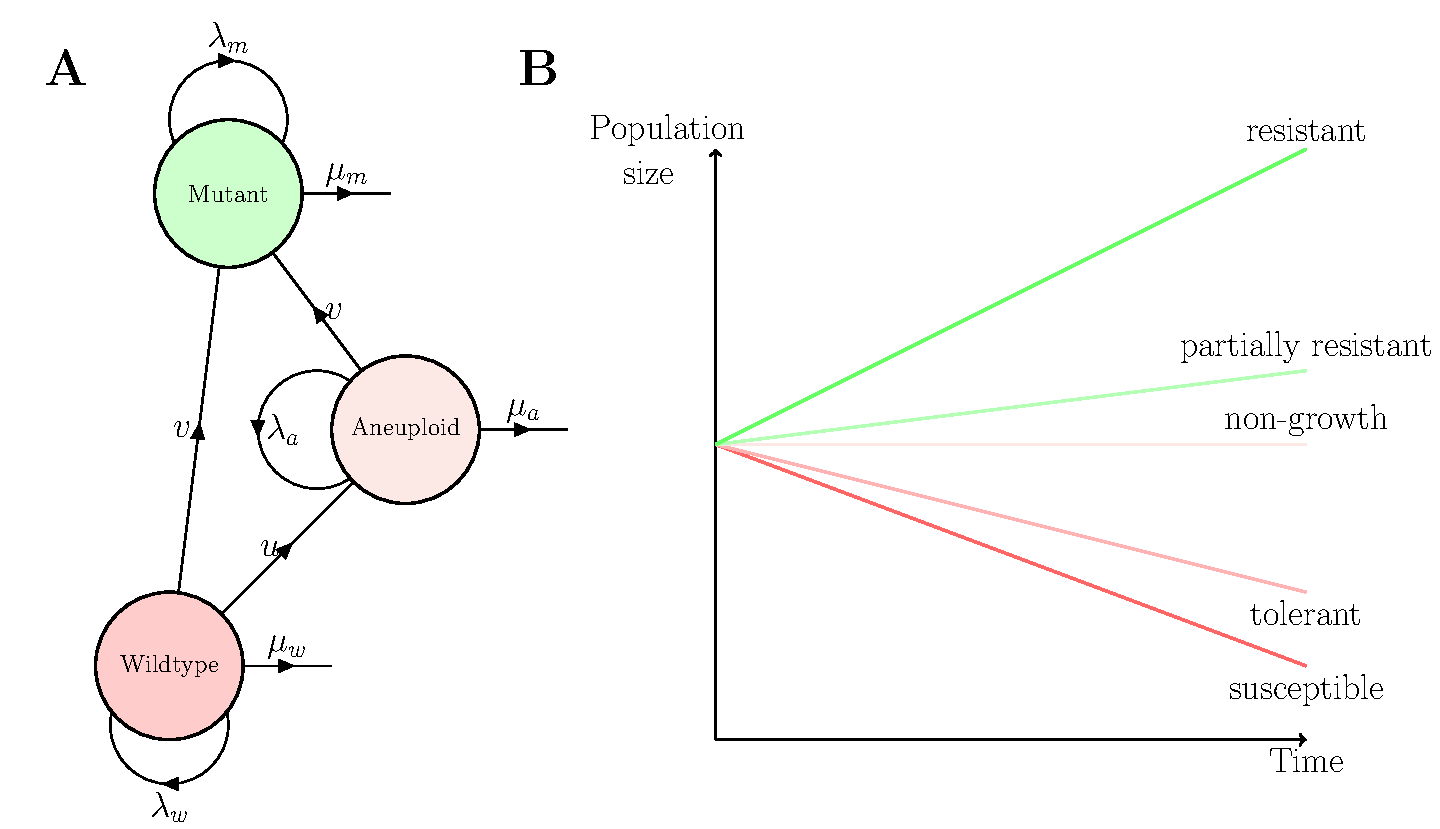
\includegraphics[width=\textwidth]{Figures/figureAneuploidy.pdf}
\caption{
\textbf{Model illustration.}
\textbf{(A)} A population of cancer cells is composed of wildtype, aneuploid, and mutant cells, which divide with rates $\lambda_w$, $\lambda_a$, and $\lambda_m$ and die at rates $\mu_w$, $\mu_a$, and $\mu_m$, respectively. 
Wildtype cells can divide and become aneuploid at rate $u\lambda_w$. Both aneuploid and wildtype cells can divide and acquire a beneficial mutation with rate $v\lambda_a$ and $v\lambda_w$, respectively. Color denotes the relative growth rates of the three genotypes such that $\lambda_w - \mu_w < \lambda_a - \mu_a < \lambda_m - \mu_m$. \textbf{(B)} The wildtype and the mutant are susceptible and resistant, respectively, to the drug. The aneuploid may be tolerant, stationary and partially resistant.
}
\label{figureAneuploidy}
\end{figure}

%%%%%%%%%%%
\begin{figure}
\begin{subfigure}{0.5\textwidth}
A\\
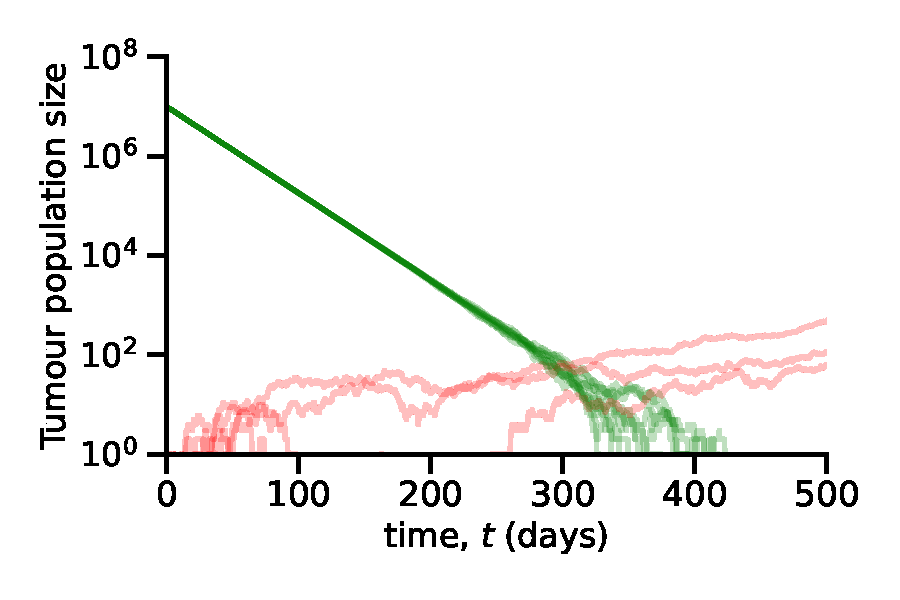
\includegraphics[width=1\textwidth]{Figures/TauLeapMeanTimeDiagramNoAneuploidy.pdf}
\end{subfigure}
\begin{subfigure}{0.5\textwidth}
B\\
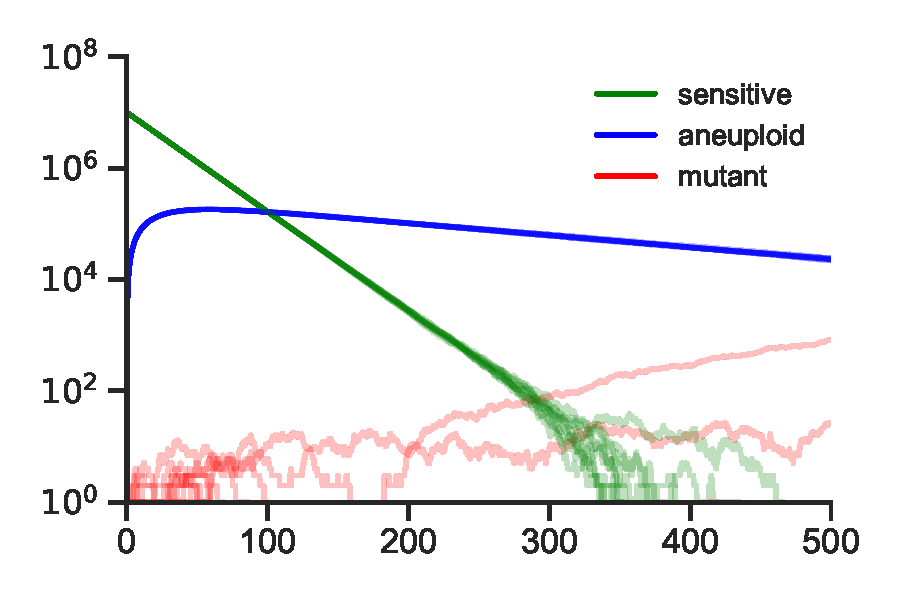
\includegraphics[width=1\textwidth]{Figures/TauLeapMeanTimeDiagramSmallda.pdf}
\end{subfigure}
\\
\begin{subfigure}{0.5\textwidth}
C\\
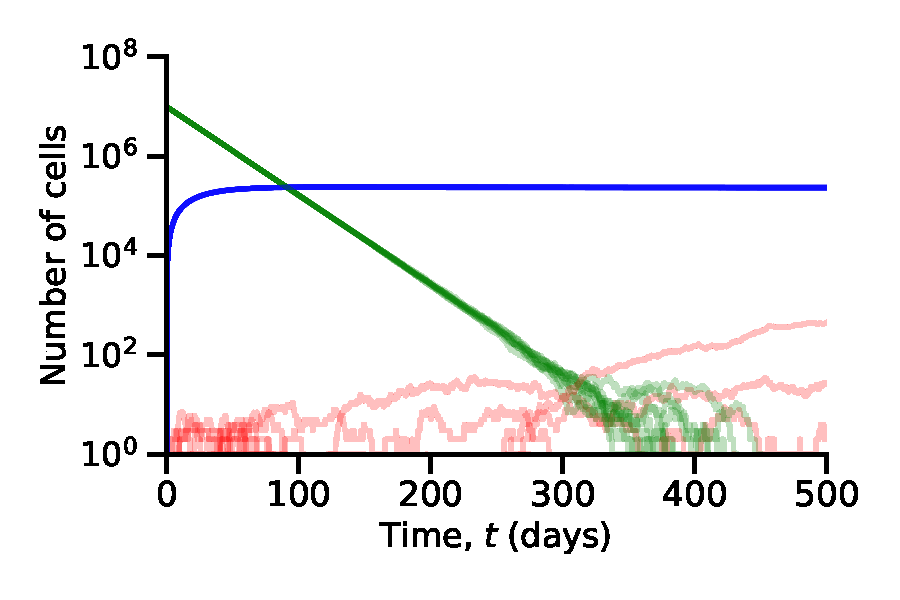
\includegraphics[width=1\textwidth]{Figures/TauLeapMeanTimeDiagramdazero.pdf}
\end{subfigure}
\begin{subfigure}{0.5\textwidth}
D\\
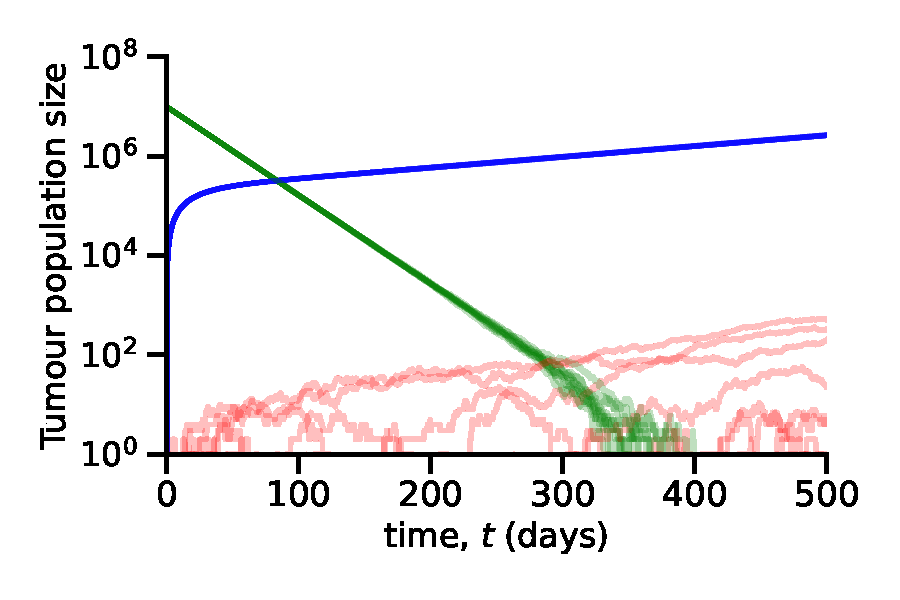
\includegraphics[width=1\textwidth]{Figures/TauLeapMeanTimeDiagramlargeda.pdf}
\end{subfigure}
\caption{
\textbf{Sample trajectories of the different genotype frequencies.}
(A) When the missegregation rate $u=0$ evolutionary rescue is only possible through direct mutation and in most cases the tumor will be killed by the drug. (B) When the aneuploidy growth rate $\Delta_a\ll0$ we observe similar dynamic to case (A) as direct mutation is the only viable route toward evolutionary rescue for the tumor. (C) Intermediate aneuploid growth rates $\Delta_a\approx0$ leads to the appearance of aneuploid lineages even after the wildtype population has gone extinct thus increasing the chance of evolutionary rescue. (D) As the growth rate of the aneuploid becomes positive we observe that the tumour is rescued by the aneuploid cancer cell population. Each plot features 10 trajectories of $\left(w_t,a_t,m_t\right)$ as a function of time $t$ for the following parameter values: $\lambda_w=0.1,\lambda_m=0.1,\mu_w=0.14,\mu_a=0.09,\mu_m=0.09, v=10^{-7},N=10^7$. For (A) we set $u=0$, for (B) $\lambda_a=0.065,u=10^{-2}$, for (C) $\lambda_a=0.0899,u=10^{-2}$ and for (D) $\lambda_a=0.095,u=10^{-2}$.
}
\label{sampleTrajectories}
\end{figure}

%%%%%%%%%%%
% Fig 3A: prob rescue vs N for various Delta_a; markup N*
% Fig 3B: N* vs Delta_a
% Fig 3C: N* vs u/v


\begin{figure}
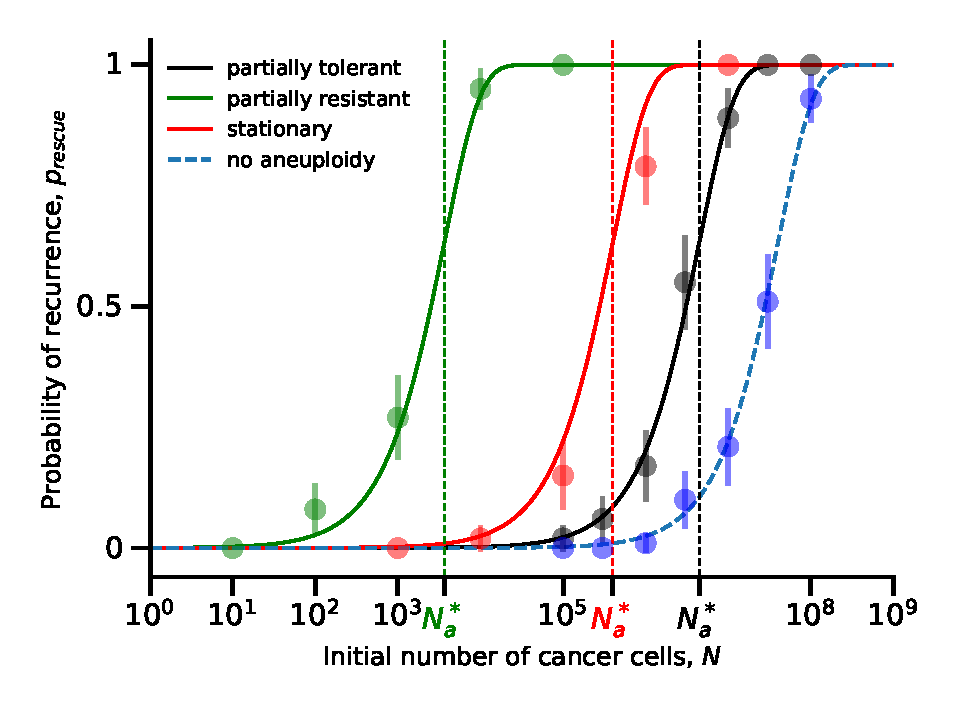
\includegraphics[width=1\textwidth]{Figures/ProbvNPlot.pdf}
\caption{\textbf{Aneuploidy facilitates evolutionary rescue of cancer under drug treatment.}
The probability of evolutionary rescue (i.e. the probability that the population does not go to extinction), $\presc$, as a function of the initial tumor size, $N$ (see \cref{eq:rescue_prob}). Dashed vertical line shows the threshold tumor size, $N_a^*$, above which the probability is very high (see \cref{eq:N_a}). Blue dashed line represents the probability of evolutionary rescue as a function of $N$ without aneuploidy ($u=0$). The black line represents the case with tolerant aneuploidy ($u=10^{-2}, \lambda_a=0.0899$), the red line represents the case with stationary aneuploidy ($u=10^{-2}, \lambda_a=0.08999$) and the green line represents the case with partially resistant aneuploidy ($u=10^{-2}, \lambda_a=0.095$). The dots represent simulations and the error bars represent $95\%$ confidence interval of the form $p\pm1.96\sqrt{p\left(1-p\right)/n}$ where $p$ is the fraction of simulations in which the tumor has adapted to the stress and $n=100$ is the number of simulations. Parameters: $\lambda_w=0.1,\lambda_m=0.1,\mu_w=0.14,\mu_a=0.09,\mu_m=0.09, v=10^{-7}$.}
\label{rescue_prob}
\end{figure}

\begin{figure}
\begin{subfigure}{0.5\textwidth}
A\\
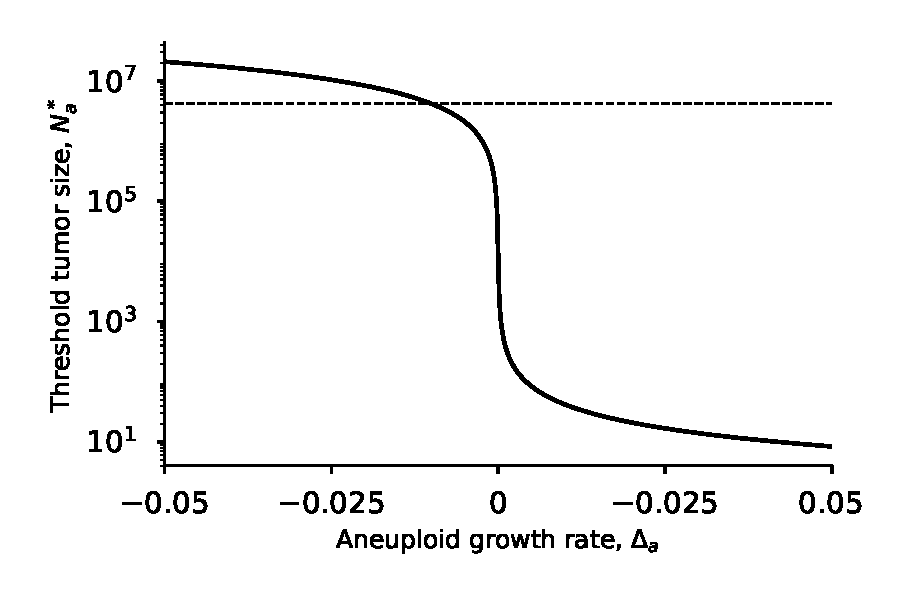
\includegraphics[width=1\textwidth]{Figures/ThresholdPopulationSizePlot.pdf}
\end{subfigure}
\begin{subfigure}{0.5\textwidth}
B\\
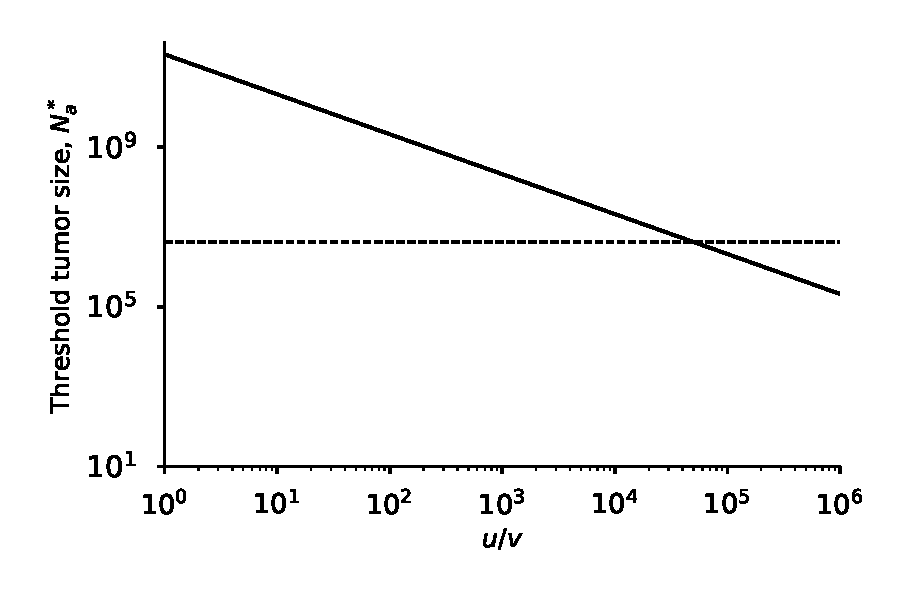
\includegraphics[width=1\textwidth]{Figures/ThresholdPopulationSizeVersusRatioPlot.pdf}
\end{subfigure}
\caption{
\textbf{Aneuploidy facilitates the evolutionary rescue of cancer under drug treatment.}
(A) The threshold tumor size $N_a^*$ as a function of the aneuploid growth rate $\Delta_a$. The dashed horizontal line shows $N^*_m$, the threshold tumor size without aneuploidy ($u=0$).  When aneuploid growth rate is close to or higher than zero, aneuploidy decreases the threshold tumor size, thereby facilitating evolutionary rescue. The inset highlights the case when aneuploidy cancer cells are non-growing. The red dots represents simulations and the error bars represent the $95\%$ confidence intervals obtained with bootstrapping, see Appendix G. Parameters: $\lambda_w=0.1,\lambda_m=0.1,\mu_w=0.14,\mu_a=0.09,\mu_m=0.09, u=10^{-2}, v=10^{-7}$.
(B) The threshold tumor size $N_a^*$ as a function of the ratio of aneuploidy and mutation rates, $u/v$. The dashed horizontal line shows $N^*_m$, the threshold tumor size without aneuploidy ($u=0$). When the aneuploidy rate is much higher than the mutation rate, aneuploidy decreases the threshold tumor size, thereby facilitating evolutionary rescue. The blue line represents the exact formula for threshold tumor size $N_a^*$ while the solid black line represents the approximation \cref{eq:N_a}. The red dots represents simulations and the error bars represent the $95\%$ confidence intervals obtained with bootstrapping, see Appendix G.  Parameters: $\lambda_w=0.1,\lambda_m=0.0899,\lambda_m=0.1,\mu_w=0.14,\mu_a=0.09,\mu_m=0.09, v=10^{-7}$. 
}
\label{rescue_threshold}
\end{figure}

%%%%%%%%%%%
% Fig 3A: N*/N* vs Delta_w 
% Fig 3B: N*/N* vs ut/s 

\begin{figure}
\begin{subfigure}{0.5\textwidth}
A\\
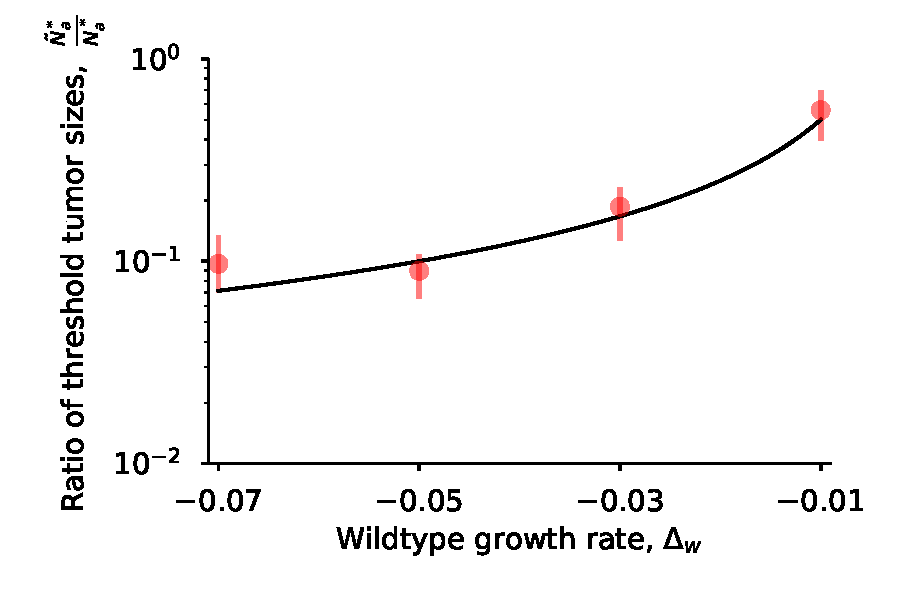
\includegraphics[width=1\textwidth]{Figures/RatiodwPlot.pdf}
\end{subfigure}
\begin{subfigure}{0.5\textwidth}
B\\
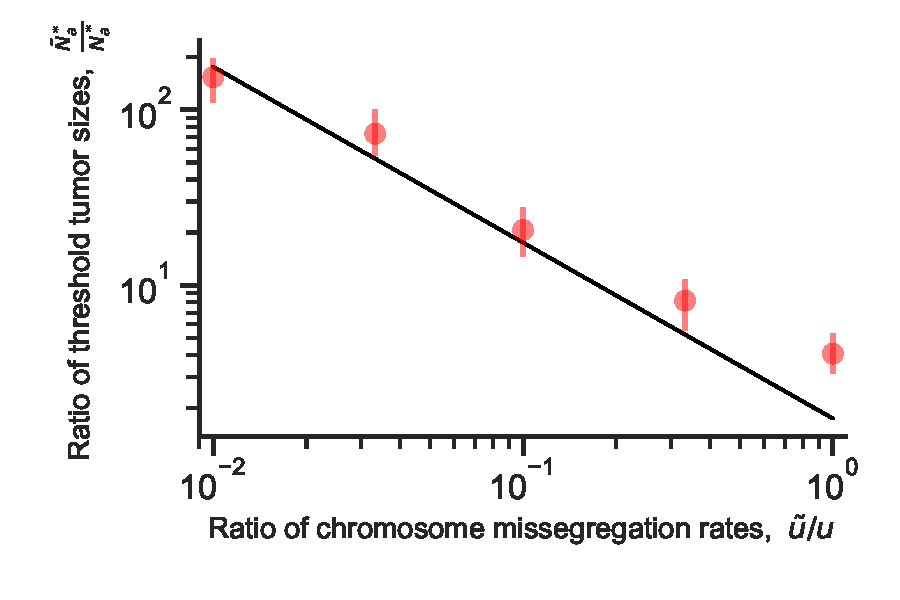
\includegraphics[width=1\textwidth]{Figures/ratio_uPlot.pdf}
\end{subfigure}
\caption{
\textbf{Standing genetic variation facilitates evolutionary rescue of cancer under drug treatment.}
(A)  The ratio of threshold tumor size $\tilde{N}_a^*$ when a fraction $\frac{\tilde{u}\lambda_w}{s}$ is aneuploid at the start of treatment and $N_a^*$ as a function of the wildtype growth rate $\Delta_w$.  Standing genetic variation will drive adaptation to the drug if $\Delta_w$ is very negative due to a stronger effect of the drug on sensitive cells. The red dots represents simulations and the error bars represent the $95\%$ confidence intervals obtained with bootstrapping, see Appendix G. Parameters: $\lambda_w=0.1,\lambda_a=0.0899,\lambda_m=0.1,\mu_a=0.09,\mu_m=0.09,\tilde{u}=10^{-3},u=10^{-2}, v=10^{-7}$.
(B) The ratio of threshold tumor size $\tilde{N}_a^*$ when a fraction $\frac{\tilde{u}\lambda_w}{s}$ is aneuploid at the start of treatment and $N_a^*$ as a function of the the ratio of aneuploidy rates $\tilde{u}/u$. De-novo aneuploids will have larger contribution to the appearance of drug resistance if the drug induces the appearance of aneuploid cells ($u \gg \tilde u$). The red dots represents  simulations and the error bars represent the $95\%$ confidence intervals obtained with bootstrapping, see Appendix G. Parameters: $\lambda_w=0.1,\lambda_a=0.0899,\lambda_m=0.1,\mu_w=0.14,\mu_a=0.09,\mu_m=0.09,\tilde{u}=10^{-3}, v=10^{-7}$.
}
\label{rescue_denovo}
\end{figure}
%%%%%%%%%%%


\begin{figure}
\vspace*{1\baselineskip}
\begin{subfigure}{0.5\textwidth}
A\\
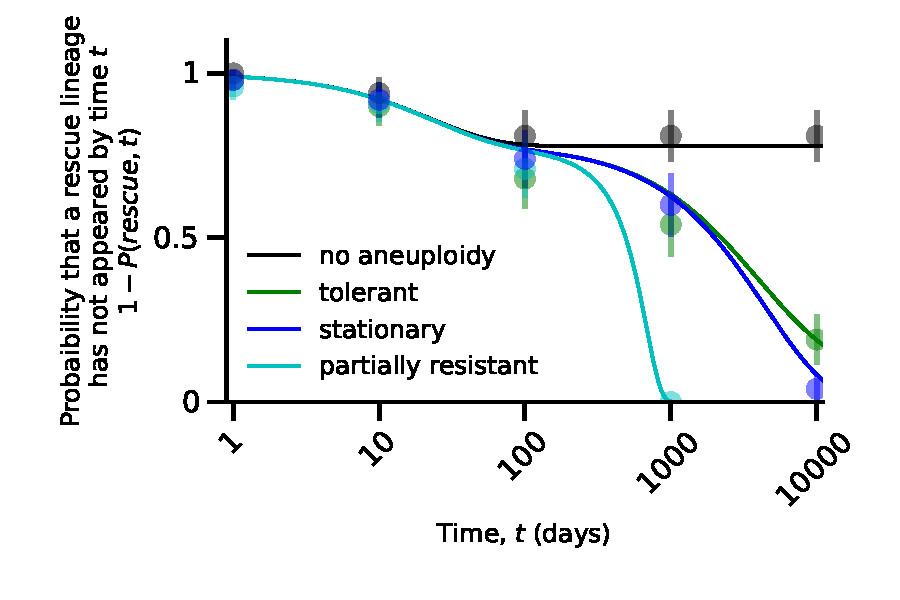
\includegraphics[width=1\textwidth]{Figures/ReboundProbability.pdf}
\end{subfigure}
\begin{subfigure}{0.5\textwidth}
B\\
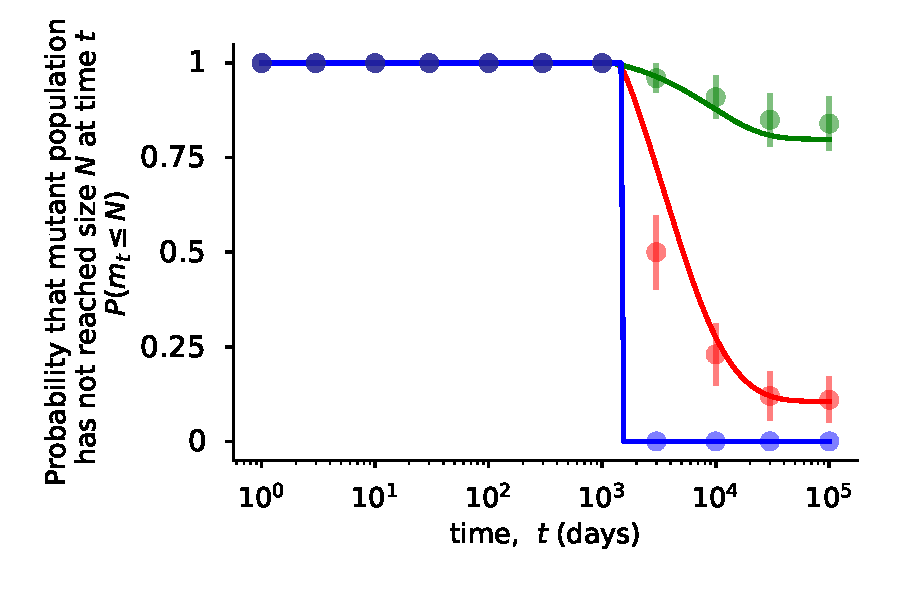
\includegraphics[width=1\textwidth]{Figures/ProliferationTimeCDFN.pdf}
\end{subfigure}
\caption{\textbf{Aneuploidy has a impact on cancer relapse early on.}
(A) The probability that a successful mutant has not appeared by time $t$. The green line represents the case with tolerant aneuploidy ($u>0, \lambda_a=0.0899$), the blue line represents the case with non-growing aneuploidy ($u>0, \lambda_a=0.089999$), the cyan line represents the case with partially resistant aneuploidy ($u>0, \lambda_a=0.095$) and the black line represents the case without aneuploidy ($u=0$).  As time increases, aneuploidy plays an important role in helping the cancer cell population escape extinction. The markers represent simulations and the error bars represent $95\%$ confidence interval of the form $p\pm1.96\sqrt{p\left(1-p\right)/n}$ where $p$ is the fraction of simulations in which a successful mutant has not been generated and $n=100$ is the number of simulations. Parameters: $\lambda_w=0.1,\lambda_m=0.1,\mu_w=0.14,\mu_a=0.09,\mu_m=0.09, u=10^{-2}, v=10^{-7},N=10^7$.
(B) The probability that a mutant cancer cell population has not reached size $N$ at time $t$. The green line represents the case where $N=10^6$ (small tumor), the red line represents $N=10^7$ (intermediate sized tumor) and the blue line represents the case where $N=10^{10}$ (large tumor). Increasing the initial tumor size guarantees that the tumor will regrow. The markers represent simulations and the error bars represents $95\%$ confidence interval of the form $p\pm1.96\sqrt{p\left(1-p\right)/n}$ where $p$ is the fraction of the simulations in which the mutant population size has not reached $N$ and $n=100$ is the number of simulations.
Parameters: $\lambda_w=0.1,\lambda_a=0.0899,\lambda_m=0.1,\mu_w=0.14,\mu_a=0.09,\mu_m=0.09, u=10^{-2}, v=10^{-7}$.}
\label{cdffig}
\end{figure}

%%%%%%%%%%%%%%%%%%%%%%%%%%%%%%%%%%%%%%%%%%

\begin{figure}
\vspace*{1\baselineskip}
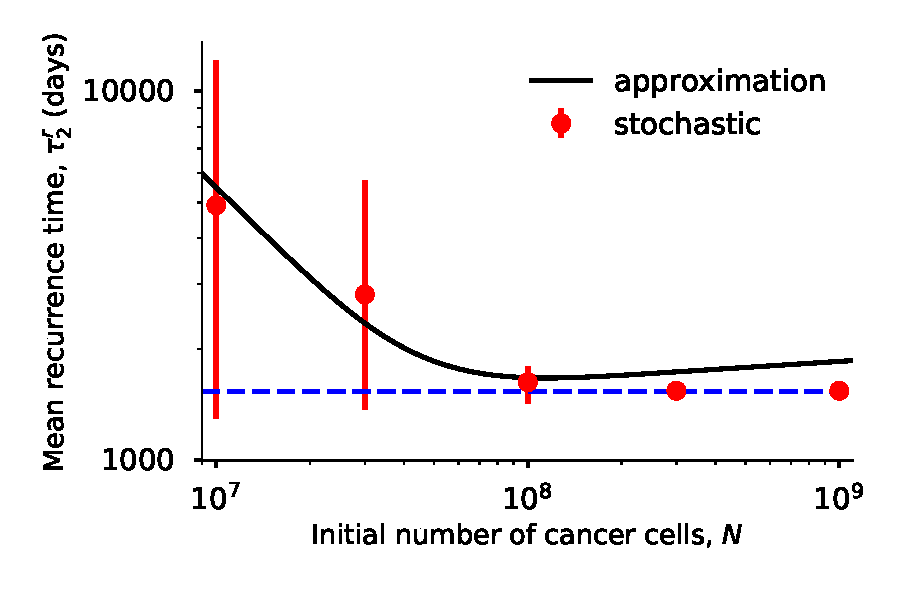
\includegraphics[width=1\textwidth]{Figures/ProliferationTime.pdf}
\caption{\textbf{Tumor size decreases the mean recurrence time.}
The mean time for the mutant cell population to reach size $N$, the initial number of cancer cells.
Our inhomogeneous Poisson-process approximation (solid black line, \cref{meanproliferationtime}) is in agreement with simulation results (red markers with 95\% confidence interval obtained with bootstrapping, see Appendix G) for intermediary $N$. The simulations converge to \cref{eq:t2det} (blue dashed line) for large values of $N$.  
Parameters: $\lambda_w=0.1,\lambda_a=0.0899,\lambda_m=0.1,\mu_w=0.14,\mu_a=0.09,\mu_m=0.09, u=10^{-2}, v=10^{-7}$.}
\label{proliferationFigure}
\end{figure}


%%%%%%%%%%%%%%%%%%%%%%%%%%%%%%%%%%%%%

\newpage 

\begin{appendices}
\renewcommand{\theequation}{\thesection\arabic{equation}}
\counterwithin*{equation}{section}


%%%%%%%%%%%%%%%%%%%%%%%%%%%%%%%%%%%%%
\section{Survival probability of a single lineage}\label{sec:appendix-surv-prob}

To analyze evolutionary rescue in this model, we use the framework of \emph{multitype branching processes} \citep{harris1963theory, weissman2009rate}. 
This allows us to find explicit expressions for the \emph{survival probability}: the probability that a lineage descended from a single cell does not become extinct.

Let $p_w$, $p_a$, and $p_m$ be the survival probabilities of a population consisting initially of single wildtype cell, aneuploid cell, or mutant cell, respectively.
The complements $1-p_w$, $1-p_a$, and $1-p_m$ are the extinction probabilities, which satisfy each its respective equation~\citep{harris1963theory},
\begin{equation} \label{eq:extinction_prob}
\begin{aligned}
1-p_w = &\frac{\mu_w}{\lambda_w+\mu_w+u\lambda_w+v\lambda_w} + 
		  \frac{u\lambda_w}{\lambda_w+\mu_w+u\lambda_w+v\lambda_w}\left(1-p_a\right)\left(1-p_w\right) + \\
		  & \frac{\lambda_w}{\lambda_w+\mu_w+u\lambda_w+v\lambda_w}\left(1-p_w\right)^2 +
		  \frac{v\lambda_w}{\lambda_w+\mu_w+u\lambda_w+v\lambda_w}\left(1-p_m\right)\left(1-p_w\right) ,\\
1-p_a = &\frac{\mu_a}{\lambda_a+\mu_a+v\lambda_a}+\frac{v\lambda_a}{\lambda_a+\mu_a+v\lambda_a}\left(1-p_m\right)\left(1-p_a\right)+\frac{\lambda_a}{\lambda_a+\mu_a+v\lambda_a}\left(1-p_a\right)^2 ,\\
1-p_m = &\frac{\mu_m}{\lambda_m+\mu_m}+\frac{\lambda_m}{\lambda_m+\mu_m}\left(1-p_m\right)^2 .	 
\end{aligned}
\end{equation}

The survival probabilities are given by the smallest solution for each quadratic equation \citep{uecker2015adaptive}. Therefore we have
\begin{equation}\label{eq:survival_prob}
\begin{aligned}
p_w &= \frac{\lambda_w-\mu_w-u\lambda_wp_a-v\lambda_wp_m+\sqrt{\left(\lambda_w-\mu_w-u\lambda_wp_a-v\lambda_wp_m\right)^2+4\lambda_w^2\left(up_a+vp_m\right)}}{2\lambda_w} ,\\
p_a &= \frac{\lambda_a-\mu_a-v\lambda_ap_m+\sqrt{\left(\lambda_a-\mu_a-v\lambda_ap_m\right)^2+4\lambda_a^2vp_m}}{2\lambda_a}, \\
p_m &= \frac{\lambda_m-\mu_m}{\lambda_m} .
\end{aligned} 
\end{equation}
Note that the equation for $p_w$ depends on both $p_a$ and $p_m$, and the equation for $p_a$ depends on $p_m$.
To proceed, we can plug the solution for $p_m$ and $p_a$ into the solution for $p_w$. We perform this for three different scenarios.

%%%%%%%%%%%%%%%%%%%%%%%%%%%%%%%%%%%%%
\subsubsection*{Scenario 1: Aneuploid cells are partially resistant} 

We first assume that aneuploidy provides partial resistance to drug therapy, $\lambda_a>\mu_a$, and that this resistance is significant, $\left(\lambda_a-\mu_a-v\lambda_ap_m\right)^2 > 4\lambda_a^2 v p_m$.
We thus rewrite \cref{eq:survival_prob} as
\begin{align*}
p_w&=\frac{\lambda_w-\mu_w-u\lambda_wp_a-v\lambda_wp_m}{2\lambda_w}\left(1-\sqrt{1+\frac{4\lambda_w^2\left(vp_m+up_a\right)}{\left(\lambda_w-\mu_w-u\lambda_wp_a-v\lambda_wp_m\right)^2}}\right) ,
\text{and} \\
p_a&=\frac{\lambda_a-\mu_a-v\lambda_ap_m}{2\lambda_a}\left(1+\sqrt{1+\frac{4\lambda_a^2vp_m}{\left(\lambda_a-\mu_a-v\lambda_ap_m\right)^2}}\right) . 
\end{align*}
Using the quadratic Taylor expansion $\sqrt{1+x}=1+x/2+\mathcal{O}(x^2)$ and assuming $u,v \ll 1$,
we obtain the following approximation for the survival probability of a population initially consisting of a single wildtype cell,
\begin{align} \label{eq:survprobwapprox1}
p_w 
&\approx -\frac{v\lambda_wp_m+u\lambda_wp_a}{\lambda_w-\mu_w-u\lambda_wp_a-v\lambda_wp_m}\\
\nonumber
&\approx-\frac{1}{\lambda_w-\mu_w}\left[\frac{u\lambda_w\left(\lambda_a-\mu_a\right)}{\lambda_a}+\frac{uv\lambda_w\lambda_a\left(\lambda_m-\mu_m\right)}{\lambda_m\left(\lambda_a-\mu_a\right)}+\frac{v\lambda_w\left(\lambda_m-\mu_m\right)}{\lambda_m}\right].
\end{align}
Now $u v$ is very small, and if we use the fact that $v \ll u$, we have:
\begin{equation}\label{eq:pw_parttolerant}
p_w \approx \frac{u\lambda_w}{\abs{\Delta_w}}  \frac{\Delta_a}{\lambda_a} .
\end{equation}
However, if aneuploidy is very rare such that
\begin{align*}
\frac{u\lambda_w\Delta_a}{\lambda_a}<\frac{v\lambda_w\Delta_m}{\lambda_m}\Rightarrow u\lambda_a<\frac{v\lambda_a^2\Delta_m}{\lambda_m} \frac{1}{\Delta_a}<\frac{v\lambda_a^2\Delta_m}{\lambda_m} \frac{1}{\sqrt{4\lambda_a^2 v p_m}}\Rightarrow u\lambda_a<T^*,
\end{align*}
where $T^* = (4 v \lambda_a^2 \Delta_m/\lambda_m)^{-1/2}$ and in the second inequality we used the fact that $\Delta_a^2 > 4\lambda_a^2 v p_m$. In this case adaptation is through direct mutation and:
\begin{equation*}
p_w \approx \frac{v\lambda_w}{\abs{\Delta_w}}  \frac{\Delta_m}{\lambda_m} .
\end{equation*}
%%%%%%%%%%%%%%%%%%%%%%%%%%%%%%%%%%%%%
\subsubsection*{Scenario 2: Aneuploid cells are tolerant.} 

We now assume that aneuploidy provides tolerance to drug therapy, that is, the number of aneuploid cells significantly declines over time, but at a lower rate than the number of wildtype cells, $\lambda_w - \mu_w < \lambda_a - \mu_a < 0$. We also assume that the decline are significant, $\left(\lambda_a-\mu_a-v\lambda_ap_m\right)^2 > 4\lambda_a^2 v p_m$.
We rewrite \cref{eq:survival_prob} as
\begin{equation}
\begin{aligned}
p_w&=\frac{\lambda_w-\mu_w-u\lambda_wp_a-v\lambda_wp_m}{2\lambda_w}\left(1-\sqrt{1+\frac{4\lambda_w^2\left(vp_m+up_a\right)}{\left(\lambda_w-\mu_w-u\lambda_wp_a-v\lambda_wp_m\right)^2}}\right), \\
p_a&=\frac{\lambda_a-\mu_a-v\lambda_ap_m}{2\lambda_a}\left(1-\sqrt{1+\frac{4\lambda_a^2vp_m}{\left(\lambda_a-\mu_a-v\lambda_ap_m\right)^2}}\right) .
\end{aligned}
\end{equation}
Since $u,v\ll1$, the term in the root can be approximated using a 1st-order Taylor expansion. So, substituting the expressions for $p_a$ and $p_m$, we have
\begin{equation} \label{eq:survprobwinitial}
\begin{aligned}
p_w&\approx-\frac{v\lambda_wp_m+u\lambda_wp_a}{\lambda_w-\mu_w-u\lambda_wp_a-v\lambda_wp_m}\\
&\approx\frac{1}{\lambda_w-\mu_w-u\lambda_wp_a-v\lambda_wp_m}\left[\frac{uv\lambda_w\lambda_a\left(\lambda_m-\mu_m\right)}{\lambda_m\left(\lambda_a-\mu_a-v\lambda_a\right)}-\frac{v\lambda_w\left(\lambda_m-\mu_m\right)}{\lambda_m}\right]\\ 
&\approx\frac{v\lambda_w\left(\lambda_m-\mu_m\right)}{\lambda_m\left(\lambda_w-\mu_w\right)}\left[\frac{u\lambda_a}{\left(\lambda_a-\mu_a\right)}-1\right] \\
&=\frac{v\lambda_w\Delta_m}{\lambda_m \abs{\Delta_w}}\left(\frac{u\lambda_a}{\abs{\Delta_a}}+1\right) .
\end{aligned}
\end{equation}
If we assume that $u\lambda_a>\abs{\Delta_a}$ then we have:
\begin{equation}\label{eq:pw_tolerant}
p_w\approx\frac{u\lambda_w}{\abs{\Delta_w}} \frac{v\lambda_a}{\abs{\Delta_a}} \frac{\Delta_m}{\lambda_m}.
\end{equation}

%%%%%%%%%%%%%%%%%%%%%%%%%%%%%%%%%%%%%
\subsubsection*{Scenario 3: Aneuploid cells are stationary} 
We now assume that the growth rate of aneuploid cells is close to zero (either positive or negative), such that  $\left(\Delta_a-v\lambda_ap_m\right)^2 \ll 4\lambda_a^2vp_m$.
We rewrite \cref{eq:survival_prob} as
\begin{equation}
p_a = \frac{\lambda_a-\mu_a-v\lambda_ap_m+2\sqrt{\lambda_a^2 vp_m}\left(1+\frac{\left(\lambda_a-\mu_a-v\lambda_ap_m\right)^2}{4\lambda_a^2vp_m}\right)^{\frac12}}{2\lambda_a} .
\end{equation}
Using a following Taylor series expansion for small $\left(\lambda_a-\mu_a-v\lambda_ap_m\right)^2 / 4\lambda_a^2vp_m$,
\begin{equation*}
\left(1+\frac{\left(\lambda_a-\mu_a-v\lambda_ap_m\right)^2}{4\lambda_a^2vp_m}\right)^{\frac{1}{2}}=1+\frac{\left(\lambda_a-\mu_a-v\lambda_ap_m\right)^2}{8\lambda_a^2vp_m}+\cdots,
\end{equation*}
we obtain the approximation
\begin{equation}
\begin{aligned}
p_a&\approx\frac{\lambda_a-\mu_a-v\lambda_ap_m+2\sqrt{\lambda_a^2 vp_m}\left[1+\frac{\left(\lambda_a-\mu_a-v\lambda_ap_m\right)^2}{8\lambda_a^2vp_m}\right]}{2\lambda_a}\\
&=\frac{\lambda_a-\mu_a-v\lambda_ap_m+2\sqrt{\lambda_a^2 vp_m}+\frac{\left(\lambda_a-\mu_a-v\lambda_ap_m\right)^2}{4\sqrt{\lambda_a^2vp_m}}}{2\lambda_a}\\
&=\frac{\left(\lambda_a-\mu_a-v\lambda_ap_m+2\sqrt{\lambda_a^2vp_m}\right)^2+4\lambda_a^2vp_m}{8\lambda_a\sqrt{\lambda_a^2vp_m}}\\
&=\frac{4\lambda_a^2vp_m+4\lambda_a^2vp_m\left(1+\frac{\lambda_a-\mu_a-v\lambda_ap_m}{2\sqrt{\lambda_a^2vp_m}}\right)^2}{8\lambda_a\sqrt{\lambda_a^2vp_m}}\\
&=\frac{1}{2\lambda_a}\left(\lambda_a-\mu_a-v\lambda_ap_m+2\sqrt{\lambda_a^2vp_m}\right).
\end{aligned}
\end{equation}
Plugging this in \cref{eq:survprobwapprox1}, the survival probability of a population starting from one wildtype individual is
\begin{equation}\label{eq:scenario3}
\begin{aligned}
p_w&\approx-\frac{1}{\lambda_w-\mu_w-u\lambda_wp_a-v\lambda_wp_m}\left[v\lambda_w\frac{\lambda_m-\mu_m}{\lambda_m}+\frac{u\lambda_w}{2\lambda_a}\left(\lambda_a-\mu_a-v\lambda_ap_m+2\sqrt{\lambda_a^2vp_m}\right)\right]\\
&=-\frac{1}{\lambda_w-\mu_w-u\lambda_w-v\lambda_w}\left[v\lambda_w\frac{\lambda_m-\mu_m}{\lambda_m}+\frac{u\lambda_w}{2\lambda_a}\left(\lambda_a-\mu_a-v\lambda_ap_m\right)+u\lambda_w\sqrt{\frac{v\left(\lambda_m-\mu_m\right)}{\lambda_m}}\right]\\
&\approx-\frac{1}{\Delta_w}\left[v\lambda_w\frac{\Delta_m}{\lambda_m}+\frac{u\lambda_w\left(\Delta_a-v\lambda_a\right)}{2\lambda_a}+u\lambda_w\sqrt{\frac{v\Delta_m}{\lambda_m}}\right].
\end{aligned}
\end{equation}
Using the fact that
\begin{equation*}
\left(\Delta_a-v\lambda_ap_m\right)^2 \ll 4\lambda_a^2vp_m\Rightarrow\frac{\Delta_a-v\lambda_ap_m}{2\lambda_a} \ll \sqrt{\frac{v\lambda_a\Delta_m}{\lambda_m}},
\end{equation*}
and $v\ll u$ we obtain:
\begin{equation}\label{eq:pw_partrest}
p_w\approx\frac{u\lambda_w}{\abs{\Delta_w}} \sqrt{\frac{v\lambda_a\Delta_m}{\lambda_m}}.
\end{equation}
%%%%%%%%%%%%%%%%%%%%%%%%%%%%%%%%%%%%%%%%%%

\section{Evolutionary rescue probability}\label{sec:appendix-rescue-prob}
Using the fact that $\Delta_a-v\lambda_ap_m\approx\Delta_a$ we write the condition $\left(\Delta_a-v\lambda_ap_m\right)^2 \ll 4\lambda_a^2vp_m$ as:
\begin{equation*}
\Delta_a^2 \ll 4\lambda_a^2vp_m\Rightarrow -1\ll\Delta_aT^*\ll1,
\end{equation*}
where $T^* = (4 v \lambda_a^2 \Delta_m/\lambda_m)^{-1/2}$.
Substituting \cref{eq:pw_parttolerant,eq:pw_partrest,eq:pw_tolerant} into \cref{eq:rescue_prob}, the evolutionary rescue probability can be approximated by
\begin{equation}\label{rescue_prob_approx}
\begin{aligned}
&\presc \approx \\
  &\begin{cases}
   1-\exp\left[-\frac{u\lambda_a}{\abs{\Delta_w}} \frac{v\lambda_w}{\abs{\Delta_a}} \frac{\Delta_m}{\lambda_m}  N\right] ,&
   \Delta_aT^*\ll-1 ,\\
   1-\exp\left[-\frac{u\lambda_w}{\abs{\Delta_w}} \sqrt{\frac{v\lambda_a\Delta_m}{\lambda_m}} N\right] ,&
  -1\ll\Delta_aT^*\ll1 ,\\
   1-\exp\left[-\frac{u\lambda_w}{\abs{\Delta_w}}  \frac{\Delta_a}{\lambda_a}  N\right] ,&
   1\ll\Delta_aT^*.
  \end{cases}
\end{aligned}
\end{equation}
%%%%%%%%%%%%%%%%%%%%%%%%%%%%%%%%%%%%%%%%%%

\section{Evolutionary rescue time}\label{sec:appendix_rescue_time}

We first calculate the expected time for the appearance of the first mutant that rescues the cell population.
This can occur either through the evolutionary trajectory $wildtype \rightarrow mutant$ or through the trajectory $wildtype \rightarrow aneuploid \rightarrow mutant$.
We start with the former. 

Assuming no aneuploidy ($u=0$), we define $T_m$ to be the time at which the first mutant cell appears that will avoid extinction and will therefore rescue the population.
Note that if extinction occurs, that is the frequency of mutants after a very long time is zero, $m_{\infty}=0$, then it is implied that $T_m=\infty$, and vice versa if $T_m<\infty$ then $m_{\infty}>0$.

The number of successful mutants generated until time $t$ can be approximated by an inhomogeneous Poisson process with rate $R_m\left(t\right) = v\lambda_w p_m w_t$,
where $w_t=N\e^{\Delta_w t}$ is the number of wildtype cells at time $t$.
Note that 
\begin{equation}\label{eq:integralR}
\int_0^{t}{R_m(z)\d z} = 
v\lambda_w p_m N \frac{\exp[{\Delta_w t}]-1}{\Delta_w} \approx 
v\lambda_w p_m N t,
\end{equation}
by integrating the exponential and because $\frac{\exp[\Delta_w t]-1}{\Delta_w}=\frac{1+\Delta_w t+\mathcal{O}(t^2)-1}{\Delta_w}=t+O(t^2)$.
The probability density function of $T_m$ is thus
$R_m\left(t\right)\exp\left(-\int_0^{t}{R_m(z)\d z}\right)$ \citep{allen2010introduction}. 
Therefore, the probability density function of the conditional random variable $(T_m \mid T_m < \infty)$ is
$f_m(t) = \frac{R_m\left(t\right)\exp\left(-\int_0^{t}{R_m(z)\d z}\right)}{\presc}$. 
\\

We are interested in the mean conditional time, $\tau_m=\mathbb{E}\left[T_m \mid T_m<\infty\right]$, which is given by
\begin{equation}\label{eq:meantime1}
\begin{aligned}
\tau_m =
\int_{0}^{\infty}{t f_m(t) \d t} = 
\frac{\int_{0}^{\infty}{tR_m(t)\exp\left(-\int_0^{t}{R_m(z)\d z}\right) \d t}}{p_{rescue}},
\end{aligned}
\end{equation}
Therefore, plugging \cref{eq:integralR,eq:rescue_prob} in \cref{eq:meantime1}, 
\begin{align}\label{eq:limitapprox_appendix}
\tau_m = 
\int_0^\infty tv\lambda_w N\e^{\Delta_wt}\frac{\e^{-v\lambda_w N p_m\frac{\e^{\Delta_w t}-1}{\Delta_w}} }{1-\left(1-p_w\right)^N} \d t\approx
\int_{0}^{\infty} tv\lambda_w N\e^{\Delta_wt}\frac{\e^{-v\lambda_w N p_mt} }{1-\e^{-Np_w}}\d t. 
\end{align}
\Cref{MeanTimeGrowthAneuploidyPlot}B show the agreement between this approximating and simulation results.
\\
Assuming aneuploidy is possible ($u>0$), we define $T_a$ to be the time at which the first mutant cell appears that will rescue the population. We are interested in the mean conditional time, $\tau_a=\mathbb{E}\left[T_a \mid T_a<\infty\right]$.

When $Nu\lambda_w/\abs{\Delta_w}\gg1$ the aneuploid frequency dynamics is roughly deterministic and therefore can be approximated by 
\begin{equation}\label{aneuploidpopeq}
a_t \approx \frac{Nu\lambda_w\e^{\Delta_wt}}{\Delta_w-\Delta_a}\left[1-\e^{-\left(\Delta_w-\Delta_a\right)t}\right].
\end{equation}
As a result, the number of successful mutants created by direct mutation and via aneuploidy can be approximated by inhomogeneous Poisson processes with the rates
\begin{align}\label{eq:twosteplineage}
r_1\left(t\right)&=v\lambda_ap_m\int_0^ta_{z} \d z = \frac{uv\lambda_w\lambda_aNp_m}{\Delta_w-\Delta_a}\left(\frac{\e^{\Delta_wt}-1}{\Delta_w}-\frac{\e^{\Delta_at}-1}{\Delta_a}\right),\\ \label{eq:twosteplineagedirect}
r_2\left(t\right)&=v\lambda_wp_m\int_0^tw_{z} \d z = v\lambda_wNp_m\frac{\e^{\Delta_w t}-1}{\Delta_w}.
\end{align}
For large initial population sizes we assume that the two processes are independent and as a result, they can be merged into a single Poisson process with rate $R_a(t)=\left(r_1+r_2\right)\left(t\right)$.
Consequently, the mean time to the appearance of the first rescue mutant is
\begin{align}\nonumber
\tau_a &= \frac{\int_{0}^{\infty}{tR_a(t)\exp\left(-\int_0^{t}{R_a(z)\d z}\right) \d t}}{p_{rescue}}\\ \label{meantimet2}
&=
\int_0^\infty t\left(v\lambda_ap_ma_t+v\lambda_wp_mw_t\right)\frac{\exp\left[-\frac{uv\lambda_w\lambda_aNp_m}{\Delta_w-\Delta_a}\left(\frac{\e^{\Delta_w t}-1}{\Delta_w}-\frac{\e^{\Delta_a t}-1}{\Delta_a}\right)-v\lambda_wNp_m\frac{\e^{\Delta_w t}-1}{\Delta_w}\right] }{1-\e^{-Np_w}}\d t,
\end{align}
which we plot in \Cref{MeanTimeGrowthAneuploidyPlot}A as a function of the initial population size, $N$.

Paradoxically, we observe from \Cref{MeanTimeGrowthAneuploidyPlot} that the mean time of a rescue mutation to appear is significantly shorter for the case when $u=0$ when compared to the case $u>0$, however this can be explained by the fact this mean time is conditioned on evolutionary rescue and, as a result, aneuploidy increase the \emph{window of opportunity} in which a rescue mutation could appear thus increasing the mean time as well (\Cref{sampleTrajectories}).

%%%
If $N\gg N_m^*$ then the mean time $\tau_a$ can be written as:
\begin{align*}
\tau_a=\int_0^\infty\e^{-R_a\left(\tau\right)}\,\d\tau=\int_0^\infty\exp\left[-\frac{uv\lambda_w\lambda_aNp_m}{\Delta_w-\Delta_a}\left(\frac{\e^{\Delta_w\tau}-1}{\Delta_w}-\frac{\e^{\Delta_a\tau}-1}{\Delta_a}\right)-v\lambda_wNp_m\frac{\e^{\Delta_w\tau}-1}{\Delta_w}\right]\,\d\tau,
\end{align*}
and we use the following Taylor series expansions:
\begin{align*}
\frac{\e^{\Delta_w\tau}-1}{\Delta_w}&=\frac{1+\Delta_w\tau+O(\tau^2)-1}{\Delta_w}=\tau+O(\tau^2).\\
\frac{\e^{\Delta_a\tau}-1}{\Delta_a}&=\frac{1+\Delta_a\tau+O(\tau^2)-1}{\Delta_a}=\tau+O(\tau^2),
\end{align*}
to obtain a simpler approximation for $\tau_a$:
\begin{align}\label{limitapprox3}
\tau_a\approx\int_0^\infty\e^{-v\lambda_wNp_m\tau}\,\d\tau=\frac{1}{v\lambda_wNp_m}.
\end{align}
If $N\ll N_a^*$ then we can write \Cref{meantimet2} as:
\begin{align}\nonumber
\tau_a&\approx\frac{\int_0^\infty tv\lambda_ap_ma_\tau\,\d\tau}{1-\e^{-Np_w}}\approx\frac{uv\lambda_a\lambda_wp_m\abs{\Delta_w+\Delta_a}}{p_w\Delta_a^2\Delta_w^2}\\ \label{limitapprox4}
&=\frac{1}{\abs{\Delta_w}}+\frac{1}{\abs{\Delta_a}},
\end{align}
where in the last line we used the fact that $1/p_w=N_a^*$ and \Cref{eq:N_a}.

If a fraction $f$ of the cancer cells are aneuploid when the drug is administered then the rates at which the rescue mutations are generated can be written as:
\begin{align*}
r_1^f\left(t\right)&=v\lambda_ap_m\int_0^ta_{z} \d z = \left(1-f\right)\frac{uv\lambda_w\lambda_aNp_m}{\Delta_w-\Delta_a}\left(\frac{\e^{\Delta_wt}-1}{\Delta_w}-\frac{\e^{\Delta_at}-1}{\Delta_a}\right)+fv\lambda_aNp_m\frac{\e^{\Delta_a t}-1}{\Delta_a},\\ 
r_2^f\left(t\right)&=v\lambda_wp_m\int_0^tw_{z} \d z = \left(1-f\right)v\lambda_wNp_m\frac{\e^{\Delta_w t}-1}{\Delta_w},
\end{align*} 
and the mean evolutionary rescue time is given by:
\begin{align}\label{meantimet2SGV}
\tau_a^f&= \frac{\int_{0}^{\infty}{tR_a^f(t)\exp\left(-\int_0^{t}{R_a^f(z)\d z}\right) \d t}}{p_{rescue}},
\end{align}
where $R_a^f(t)=r_1^f\left(t\right)+r_2^f\left(t\right)$ and $p_{rescue}=1-\exp\left[-\left(1-f\right)p_wN-fp_aN\right]$. We plot our approximation in  \Cref{SGVEvolutionaryRescueTimeComplete} together with simulated data.
%%%%%%%%%%%%%%%%%%%%%%%%%%%%%%%%%%%%%%%%%%

\section{Recurrence time}\label{sec:appendix_recurrence_time}
We define the proliferation time $\tau_a^r$  to be the time it takes the population of mutant cancer cells to reach the initial tumor size $N$. The number of rescue lineages generated by the wildtype population is given by  \cref{eq:twosteplineage} (see \Cref{ExpectedNumberRescueLineages}):
\begin{equation*}
r_1\left(\infty\right)=\frac{uv\lambda_w\lambda_aNp_m}{\abs{\Delta_w}\abs{\Delta_a}}=\frac{N}{N_a^*},
\end{equation*}
where we ignore lineages created by direct mutation because we assumed $u\lambda_a > \max{(-\Delta_a, 1/T^*)}$, $N\ll N_m^*$ and used \Cref{eq:N_a}.

This helps us distinguish between two cases for the proliferation time. Firstly, when we have at most one lineages which rescues the cancer cell population:
\begin{equation*}
N\ll N_a^*.
\end{equation*}
As a result, the recurrence time is given by~\citep{avanzini2019cancer}:
\begin{align}\label{meanproliferationtime}
\tau_a^r&\approx\tau_a+\frac{\log p_mN}{\Delta_m}.
\end{align}
The factor of $p_m$ in the second term of \cref{meanproliferationtime} is due to the fact that the lineage is conditioned to survive genetic drift and the time to reach $N$ is shorter then the case without this property. 

The second case is when the wildtype population produces a large number of rescue lineages in a short period of time. This is given by the condition:
\begin{align*}
N\gg N_a^*.
\end{align*}
As a result, the recurrence time is obtained by solving the following system of ODEs:
\begin{equation}\label{detODE}
\begin{aligned}
\frac{dw}{dt}&=\Delta_ww,\\
\frac{da}{dt}&=\Delta_aa+u\lambda_ww,\\
\frac{dm}{dt}&=\Delta_mm+v\lambda_aa+v\lambda_ww.
\end{aligned}
\end{equation}
Solving the system of ODEs for initial condition $\left(w(0), a(0), m(0)\right)=\left(N,0,0\right)$ we obtain:
\begin{align*}
m\left(t\right)=\frac{Nuv\lambda_a\lambda_w}{\Delta_w-\Delta_a}\left[\frac{\e^{\Delta_wt}-\e^{\Delta_mt}}{\Delta_w-\Delta_m}-\frac{\e^{\Delta_at}-\e^{\Delta_mt}}{\Delta_a-\Delta_m}\right]+Nv\lambda_w\frac{\e^{\Delta_wt}-\e^{\Delta_mt}}{\Delta_w-\Delta_m}.
\end{align*}
We obtain $\tau_a^r$ such that $m\left(\tau_a^r\right)=N$ by solving:
\begin{equation}%\label{eq:t2det}
1=\frac{uv\lambda_a\lambda_w}{\Delta_w-\Delta_a}\left[\frac{\e^{\Delta_w\tau_a^r}-\e^{\Delta_m\tau_a^r}}{\Delta_w-\Delta_m}-\frac{\e^{\Delta_a\tau_a^r}-\e^{\Delta_m\tau_a^r}}{\Delta_a-\Delta_m}\right]+v\lambda_w\frac{\e^{\Delta_w\tau_a^r}-\e^{\Delta_m\tau_a^r}}{\Delta_w-\Delta_m}.
\end{equation}
This is a transcendental equation which cannot be solved exactly but we can obtain an approximation by noting that for large $\tau_a^r$ the above equation can be written as: 
\begin{equation*}
1=v\lambda_w\frac{\e^{\Delta_m\tau_a^r}}{\abs{\Delta_w-\Delta_m}},
\end{equation*}
which has solution:
\begin{equation}\label{eq:t2det}
\tau_a^r\approx\frac{1}{\Delta_m}\log\frac{\Delta_m-\Delta_w}{v\lambda_w}.
\end{equation}
We observe that the terms given by the evolutionary trajectory $wildtype \rightarrow aneuploid \rightarrow mutant$ do not contribute to the above approximation and, as a result, we deduce that it accurate only for $N\gg N_m^*>N_a^*$.

Additionally, we note that if we are interested in the time until the tumor reaches a detectable size $M$ then our above analysis is valid but in \Cref{meanproliferationtime} we change:
\begin{align}\label{meanproliferationtime2}
\tau_a^{r,M}&\approx\tau_a+\frac{\log p_mM}{\Delta_m},
\end{align}
and \Cref{eq:t2det} becomes:
\begin{equation}\label{eq:t2det2}
\tau_a^{r,M}\approx\frac{1}{\Delta_m}\log\frac{M\left(\Delta_m-\Delta_w\right)}{v\lambda_wN},
\end{equation}
which we plot in \Cref{RecurrencePlot} and observe that our approximations are in agreement with simulations.
%%%%%%%%%%%%%%%%%%%%%%%%%%%%%%%%%%%%%%%%%%

\section{Distribution of evolutionary rescue time}\label{sec:appendix_distribution_time}
The probability that a successful mutant has been generated by time $t$ is given by:
\begin{align*}
P\left(rescue,t\right)&=P\left(T_a<t\right)\\
&=1-\exp\left\{-\left[r_1\left(t\right)+r_2\left(t\right)\right]\right\}\\
&=1-\exp\left\{-\left[\frac{uv\lambda_w\lambda_aNp_m}{\Delta_w-\Delta_a}\left(\frac{\e^{\Delta_wt}-1}{\Delta_w}-\frac{\e^{\Delta_at}-1}{\Delta_a}\right)+ v\lambda_wNp_m\frac{\e^{\Delta_w t}-1}{\Delta_w}\right]\right\},
\end{align*}
where $T_a$ is the time at which the first mutant cell appears that will avoid extinction and which was defined in appendix \ref{sec:appendix_rescue_time}.

As a result, the probability that a successful mutant has not been generated by time $t$ is:
\begin{equation}
1-P\left(rescue,t\right)=\exp\left\{-\left[\frac{uv\lambda_w\lambda_aNp_m}{\Delta_w-\Delta_a}\left(\frac{\e^{\Delta_wt}-1}{\Delta_w}-\frac{\e^{\Delta_at}-1}{\Delta_a}\right)+ v\lambda_wNp_m\frac{\e^{\Delta_w t}-1}{\Delta_w}\right]\right\}.
\end{equation}
%%%%%%%%%%%%%%%%%%%%%%%%%%%%%%%%%%%%%%%%%
\section{Distribution of recurrence time}
The probability distribution of the time that a lineage, consisting initially of a single cell, will reach size $N$ as time $t$ is given by the Gumbel distribution $\text{Gumb}_{max}\left(\frac{\log Np_m}{\Delta_m},\frac{1}{\Delta_m}\right)$~\citep{avanzini2019cancer} with probability density function:
\begin{align*}
G\left(t\right)=\e^{-p_mN\e^{-\Delta_mt}}.
\end{align*}
A mutant lineage initiated at time $s$, through aneuploidy, at rate $v\lambda_ap_ma_s$ reaches size $N$ before time $t$ with probability $G\left(t-s\right)$ where $s\leq t$. As a result, the number of successful mutant lineages which reach size $N$ by time $t$ can be approximated by inhomogeneous Poisson random variable with rate:
\begin{align*}
r\left(t\right)=v\lambda_ap_m\int_0^t a_sG\left(t-s\right)\,\d s
\end{align*}
where $a_s$ is aneuploid population size at time $s$ defined in \cref{aneuploidpopeq}. The proliferation time is defined as the first time the size of all lineages reaches $N$. When $N\ll\abs{\Delta_w}\abs{\Delta_a}/uv\lambda_w\lambda_ap_m$ there is at most a single mutant lineage that will survive and reach size $N$ (\Cref{ExpectedNumberRescueLineages}) and the probability that the size of that lineage has not reached $N$ by time $t$ is given by:
\begin{align}\nonumber
P\left(m_t\leq N\right)&=\exp\left[-r\left(t\right)\right]\\ \label{eqmNs}
&=\exp\left[-\frac{Nuv\lambda_w\lambda_ap_m}{\Delta_w-\Delta_a}\int_0^t\left[\e^{\Delta_ws}-\e^{\Delta_as}\right]\e^{-p_mN\e^{-\Delta_m\left(t-s\right)}}\,\d s\right].
\end{align}
When $N\gg\abs{\Delta_w}\abs{\Delta_a}/uv\lambda_w\lambda_ap_m$ the dynamics of the cancer cell populations is deterministic and approximated by the system of ODEs shown in \cref{detODE}. As a result, the size of the mutant cell population will always be below $N$ until time $\tau_a^r$ and will always be greater after:
\begin{align}\label{eqmNd}
P\left(m_t\leq N\right)=1-H\left(t-\tau_a^r\right),
\end{align}
where $H(x)$ is the Heaviside function:
\begin{equation*}
H\left(x\right) = \begin{cases}
    0 ,&
  x<0 ,\\ 
  1 ,&
  x\geq0 .
  \end{cases}
\end{equation*}
We plot \cref{eqmNs} and \cref{eqmNd} in Figure and compare with stochastic simulations and observe that our approximation are in agreement. 

We observe that for $N=10^7$ our formula overestimates the probability that the mutant population will be smaller then $N$ at time $t$.  This can be explained by the fact that $N=10^7$ is an intermediary case where the wildtype population produces a number of rescue lineages that is greater then one but still sufficiently small such that stochasticity plays an important role in the population dynamics. As a result, the number of mutant cancer cells will reach $N$ faster then the case with a single mutant lineage. Additionally, we observe from \Cref{cdffig}B that the probability of the mutant cell population reaching size $N$ is approximately zero before time $\tau_a^r$ which is the recurrence time for the deterministic case. This can be explained as follows: in the deterministic case there is a sufficient number of lineages produced such that there exists a lineage where each descendant will only reproduce and not die; the time it takes for this lineage to reach $N$ is the lower bound for the time of all other lineages to reach $N$ and this time cannot be smaller then $\tau_a^r$ by definition. Given that for small values of $N$ we expect that at most a single lineage will rescue the tumor, this lineage cannot reach $N$ before $\tau_a^r$ for the deterministic case \cref{eq:t2det}.

From  \cref{eqmNd} we obtain the distribution of the recurrence time conditional of evolutionary rescue:
\begin{align}\label{distribution}
f\left(t\right)&=\frac{d}{dt}\left[\frac{P\left(m_t\geq N\right)}{p_{rescue}}\right]=r'\left(t\right)\frac{\exp\left[-r\left(t\right)\right]}{p_{rescue}},
\end{align}
which we plot in \Cref{KMdistribution} and compare with simulations. We note that in the case $N\gg\abs{\Delta_w}\abs{\Delta_a}/uv\lambda_w\lambda_ap_m$ the distribution becomes the Dirac $\delta$-function~\citep{barton1989elements}.
%%%
\section*{Appendix G: Bootstrapping}
For the mean times the $95\%$ confidence interval is obtained through bootstrapping in the following steps: (1) we simulate $T$ 100 times; (2) we sample with replacement which we store in $T'$; (3) for each element of this sample we obtain $\tau=\mathbb{E}\left[T'\right]$; (4) we repeat steps (2)-(3) 100 times to obtain $\tau$ and we select the upper and lower limits such that $95\%$ of the values of $\tau$ lie in the interval given by the bounds.

For the threshold tumor sizes the $95\%$ confidence interval is obtained through bootstrapping in the following steps: (1) we simulate $p_{rescue}$ 100 times; (2) we sample with replacement which we store in $S$; (3) for each element of this sample we obtain $N_a^*=1/p_w$ using $p_w=-1/N_s\log\left(1-\bar{S}\right)$ where $\bar{S}$ is the mean of $S$ and $N_s$ is an arbitrary value of the initial population size we selected in order to calculate $p_{rescue}$; (4) we repeat steps (2)-(3) 100 times to obtain $N_a^*$ and we select the upper and lower limits such that $95\%$ of the values of $N_a^*$ lie in the interval given by the bounds.

For the ratio of the threshold tumor sizes the $95\%$ confidence interval is obtained through bootstrapping in the following steps: (1) we simulate $p_{rescue}$ 100 times for both the case when $f=\tilde{u}\lambda_w/s$ and $f=0$; (2) we sample with replacement which we store in $S_0$ and  $S_f$; (4) for each element of $S_0$ we obtain $N_a^*=1/p_w$ using $p_w=-1/N_s\log\left(1-\bar{S}\right)$ where $\bar{S}$ is the mean of $S_0$ and $N_s$ is an arbitrary value of the initial population size we selected in order to calculate $p_{rescue}$; (5) for each element of $S_f$ we obtain $\tilde{N}_a^*=1/p_a$ using $p_a=-f/N_s\log\left(1-\bar{S}\right)$ where $\bar{S}_f$ is the mean of $S_f$ and $N_s$ is an arbitrary value of the initial population size we selected in order to calculate $p_{rescue}$; (6) we repeat steps (2)-(5) 100 times to obtain $\tilde{N}_a^*/N_a^*$ and we select the upper and lower limits such that $95\%$ of the values of $\tilde{N}_a^*/N_a^*$ lie in the interval given by the bounds.
%%%%%%%%%%%%%%%%%%%%%%%%%%%%%%%%%%%%%%%%%

\newpage
\section*{Supplementary Figures}
\beginsupplement % https://support.authorea.com/en-us/article/how-to-create-an-appendix-section-or-supplementary-information-1g25i5a/

\begin{figure}[h]
\vspace*{1\baselineskip}
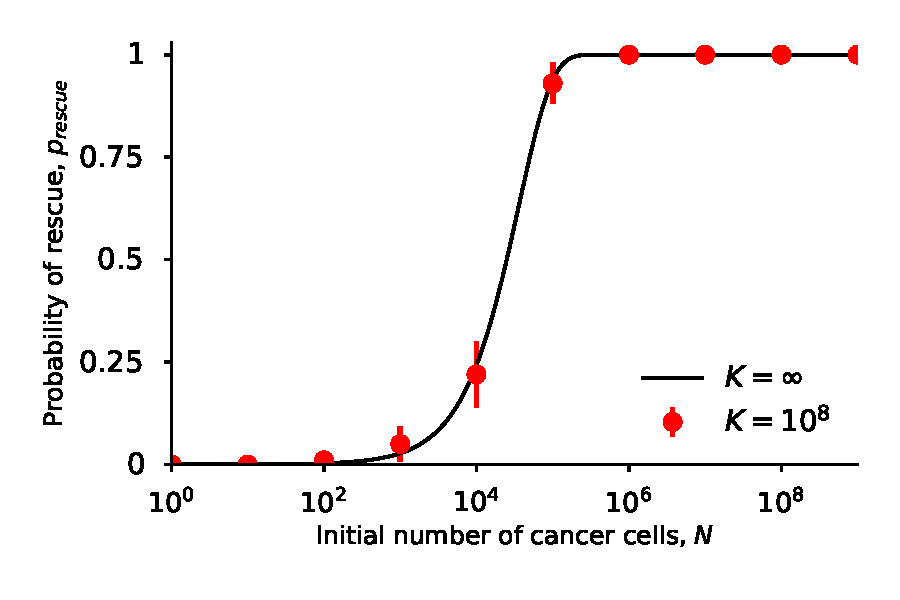
\includegraphics[width=1\textwidth]{Figures/SurvPlotNDataLogisticK.pdf}
\caption{\textbf{Density dependent growth does not affect the accuracy of our model.} Comparison of results of simulations  with density-dependent growth (red markers with with 95\% CI) and the approximation formula (black line, \cref{eq:N_a} in \cref{eq:rescue_prob}) with maximum carrying capacity $K=10^8$ and effective carrying capacity $K_e=K\Delta_a/\lambda_a\approx10^6$. The error bars represent $95\%$ confidence interval of the form $p\pm1.96\sqrt{p\left(1-p\right)/n}$ where $p$ is the  fraction of simulations in which the tumor has adapted to the stress and $n=100$ is the number of simulations. Parameters: $\lambda_w=0.1,\lambda_a=0.0901,\lambda_m=0.1,\mu_w=0.14,\mu_a=0.09,\mu_m=0.09, u=10^{-2}, v=10^{-7}, K=10^8$.}
\label{LogisticPlot}
\end{figure}
%%%
\begin{figure}[!htb]
\begin{subfigure}{0.5\textwidth}
A\\
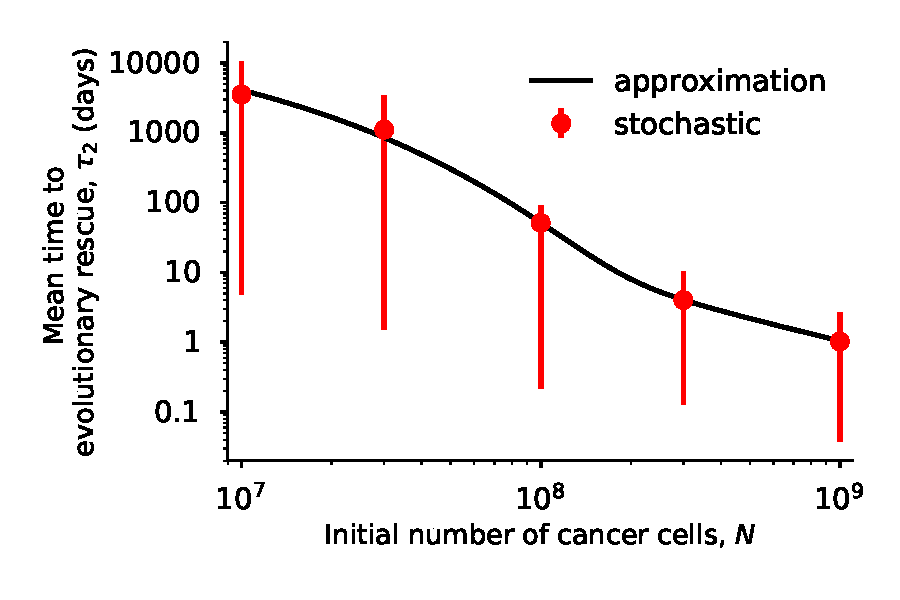
\includegraphics[width=1\textwidth]{Figures/EvolutionaryRescueTime.pdf}
\end{subfigure}
\begin{subfigure}{0.5\textwidth}
B\\
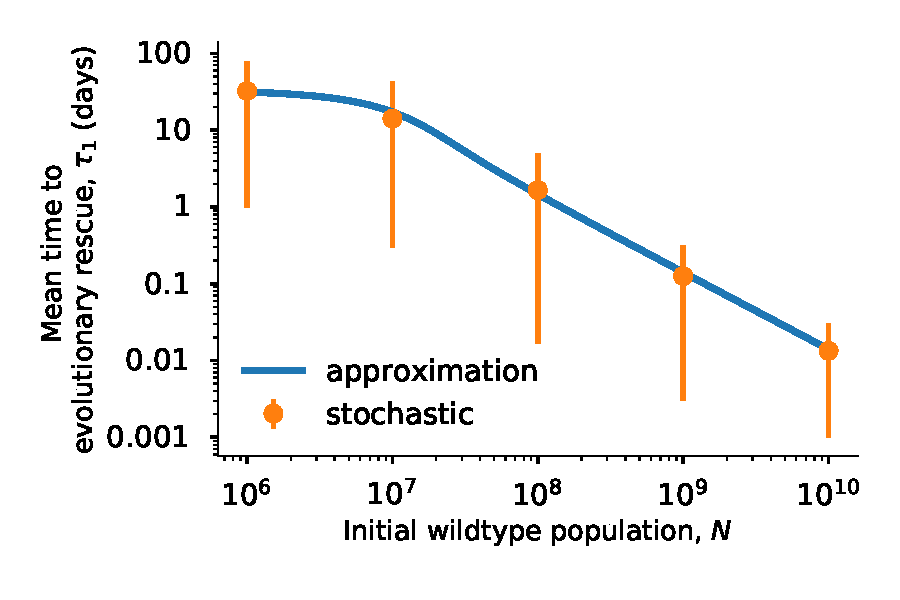
\includegraphics[width=1\textwidth]{Figures/MeanTimeGrowthMutantDirectPlot.pdf}
\end{subfigure}
\caption{\textbf{Evolutionary rescue time.}
Shown is the mean time for appearance of a resistance mutation the leads to evolutionary rescue (A) with aneuploidy ($u>0$) and (B) without aneuploidy ($u=0$).
Our inhomogeneous Poisson-process approximations (solid black lines, right: \cref{eq:meantime1}, left: \cref{meantimet2}) is in agreement with simulation results (red markers with 95\% quantile intervals obtained with bootstrapping, see see Appendix G). 
Parameters: $\lambda_w=0.1,\lambda_m=0.0899,\lambda_m=0.1,\mu_w=0.14,\mu_a=0.09,\mu_m=0.09, u=10^{-2}, v=10^{-7}$.
}
\label{MeanTimeGrowthAneuploidyPlot} 
\end{figure}
%%%
\begin{figure}
\vspace*{1\baselineskip}
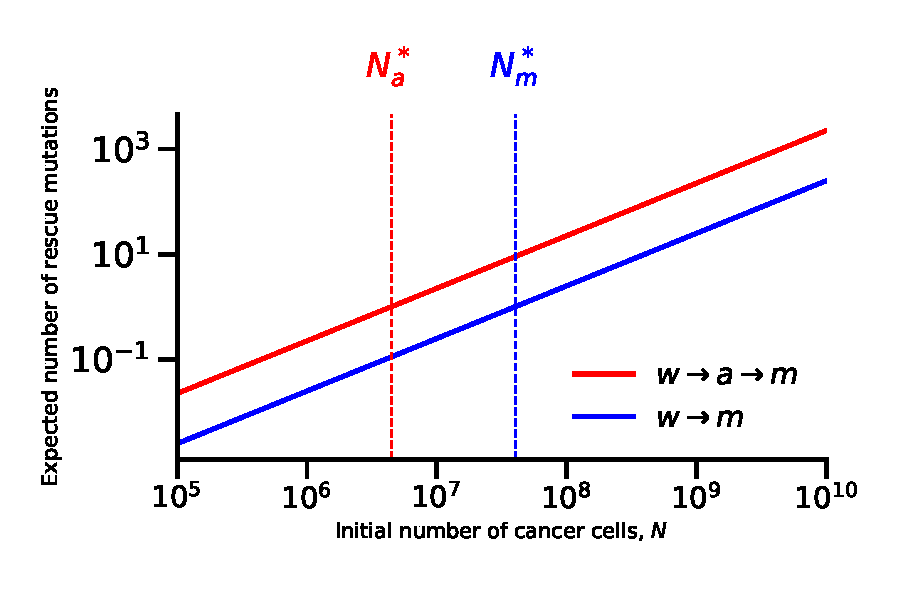
\includegraphics[width=1\textwidth]{Figures/ExpectedNumber.pdf}
\caption{\textbf{Aneuploidy increases the number of mutations which rescue the tumor.} Shown is the expected number of mutation, which will rescue the cancer cell population, produced through the evolutionary trajectory $wildtype \rightarrow mutant$ (blue line, \cref{eq:twosteplineagedirect}) or through the trajectory $wildtype \rightarrow aneuploid \rightarrow mutant$ (red line, \cref{eq:twosteplineage}).
Parameters: $\lambda_w=0.1,\lambda_m=0.0899,\lambda_m=0.1,\mu_w=0.14,\mu_a=0.09,\mu_m=0.09, u=10^{-2}, v=10^{-7}$.}
\label{ExpectedNumberRescueLineages}
\end{figure}
%%%
\begin{figure}
\vspace*{1\baselineskip}
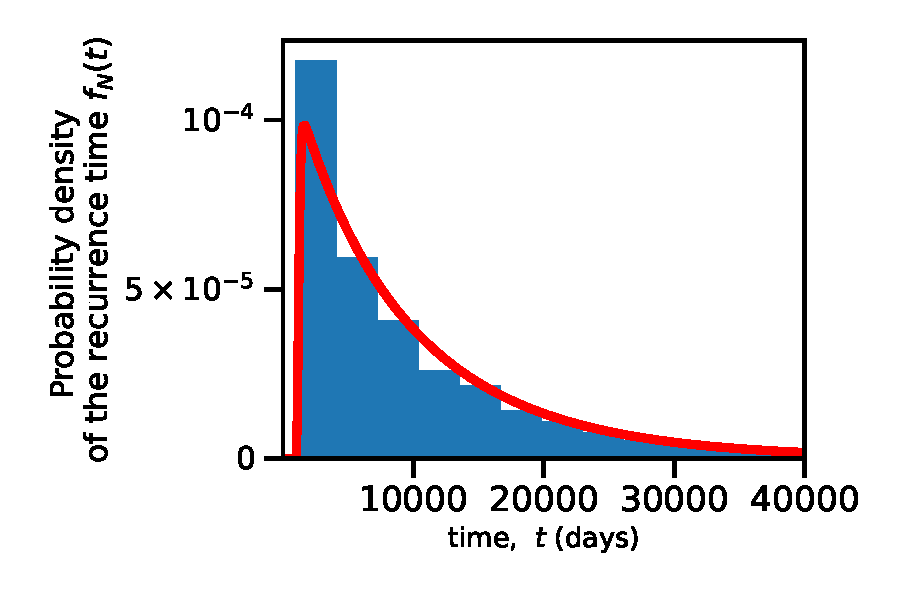
\includegraphics[width=1\textwidth]{Figures/KaplanMeierDistribution.pdf}
\caption{\textbf{Distribution of the recurrence time.}
Shown is the distribution of the time for the mutant cell population to reach size $N$, where $N$ is the initial number of cancer cells. The red line is analytic result \cref{distribution} overlaid over the histogram of simulations. 
Parameters: $N=10^6, \lambda_w=0.1,\lambda_a=0.0899,\lambda_m=0.1,\mu_w=0.14,\mu_a=0.09,\mu_m=0.09, u=10^{-2}, v=10^{-7}$.}
\label{KMdistribution}
\end{figure}
%%%
\begin{figure}
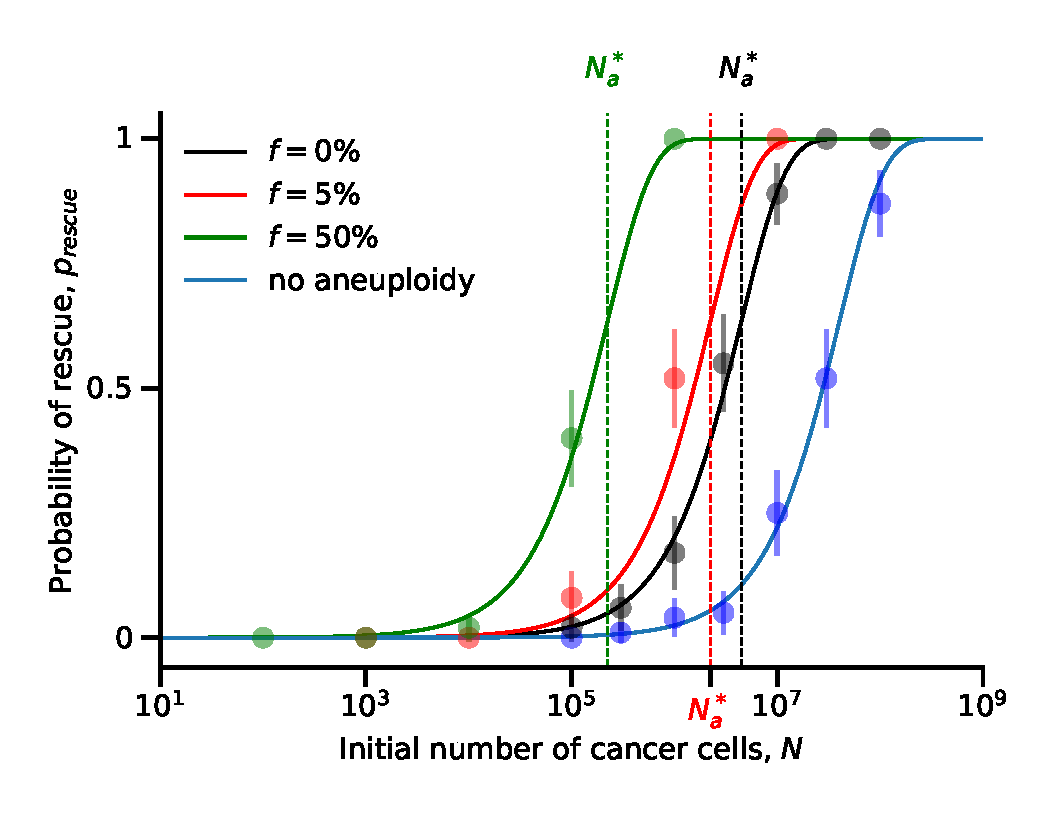
\includegraphics[width=1\textwidth]{Figures/ProbvN_SGV_Plot.pdf}
\caption{The probability of evolutionary rescue (i.e. the probability that the population does not go to extinction), $\presc$, as a function of the initial tumor size, $N$. Dashed vertical line shows the threshold tumor size, above which the probability is very high. Blue dashed line represents the probability of evolutionary rescue as a function of $N$ without aneuploidy ($u=0$). The black line represents the case where a fraction $f=0\%$ of the initial tumor is aneuploid, the red line represents the case with $f=5\%$ and the green line represents the case with $f=50\%$. The dots represent simulations and the error bars represent $95\%$ confidence interval of the form $p\pm1.96\sqrt{p\left(1-p\right)/n}$ where $p$ is the fraction of simulations in which the tumor has adapted to the stress and $n=100$ is the number of simulations. Parameters: $\lambda_w=0.1,\lambda_a=0.0899,\lambda_m=0.1,\mu_w=0.14,\mu_a=0.09,\mu_a=0.09,\mu_m=0.09, u=10^{-2}, v=10^{-7}$.}
\label{rescue_prob_sgv}
\end{figure}
%%%
\begin{figure}
\vspace*{1\baselineskip}
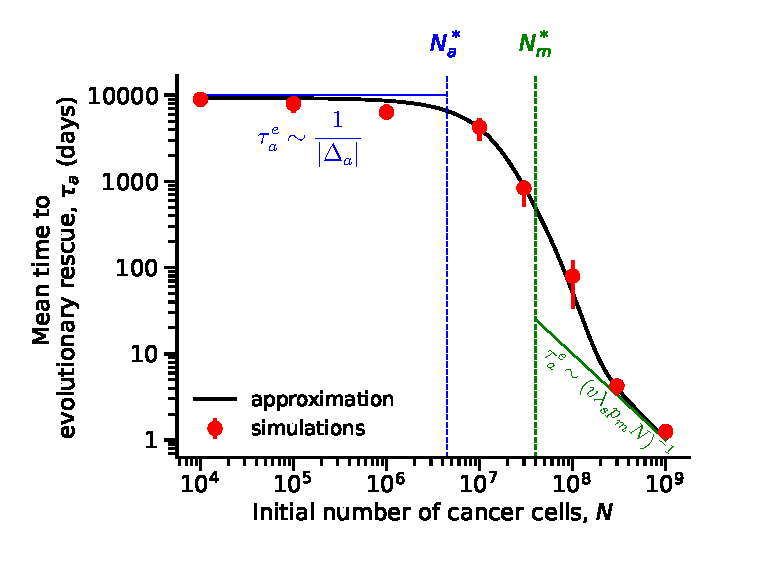
\includegraphics[width=1\textwidth]{Figures/EvolutionaryRescueTimeComplete.pdf}
\caption{Shown is the mean time for appearance of a resistance mutation the leads to evolutionary rescue with aneuploidy ($u>0$). Our inhomogeneous Poisson-process approximations (solid black lines, right: \cref{meantimet2}) is in agreement with simulation results (red markers with 95\% confidence intervals obtained with bootstrapping, see Appendix G). Dashed vertical blue line represents the threshold tumor size above which evolutionary rescue is very likely through aneuploidy \cref{eq:N_a} and the dashed vertical green line represents the threshold tumor size above which evolutionary rescue is very likely through direct mutation \cref{eq:N_m}. Solid lines represents the approximations \cref{eq:AsymptoticTimeRules} ($N<N_a^*$ blue line and $N>N_m^*$ green line). 
Parameters: $\lambda_w=0.1,\lambda_m=0.0899,\lambda_m=0.1,\mu_w=0.14,\mu_a=0.09,\mu_m=0.09, u=10^{-2}, v=10^{-7}$.}
\label{EvolutionaryRescueTimeComplete}
\end{figure}
%%%
\begin{figure}
\vspace*{1\baselineskip}
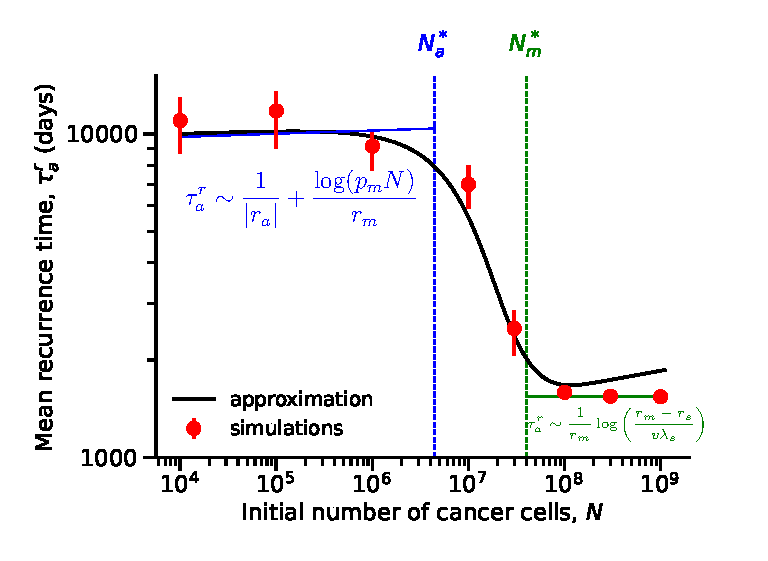
\includegraphics[width=1\textwidth]{Figures/ProliferationTimeLarge.pdf}
\caption{The mean time for the mutant cell population to reach size $N$, where $N$ is the initial number of cancer cells.
Our inhomogeneous Poisson-process approximation (solid black line, \cref{meanproliferationtime}) is in agreement with simulation results (red markers with 95\% confidence intervals obtained with bootstrapping, see Appendix G) for small and intermediate values of $N$. Dashed vertical blue line represents the threshold tumor size above which evolutionary rescue is very likely through aneuploidy \cref{eq:N_a} and the dashed vertical green line represents the threshold tumor size above which evolutionary rescue is very likely through direct mutation \cref{eq:N_m}. Solid lines represents the approximations \cref{eq:AsymptoticTimeRulesRecurrence} ($N<N_a^*$ blue line and $N>N_m^*$ green line). The simulations converge to \cref{eq:t2det} (green line) for large values of $N\gg N_m^*$.  Parameters: $\lambda_w=0.1,\lambda_a=0.0899,\lambda_m=0.1,\mu_w=0.14,\mu_a=0.09,\mu_m=0.09, u=10^{-2}, v=10^{-7}$.}
\label{ProliferationTimeLarge}
\end{figure}
%%%
\begin{figure}
\vspace*{1\baselineskip}
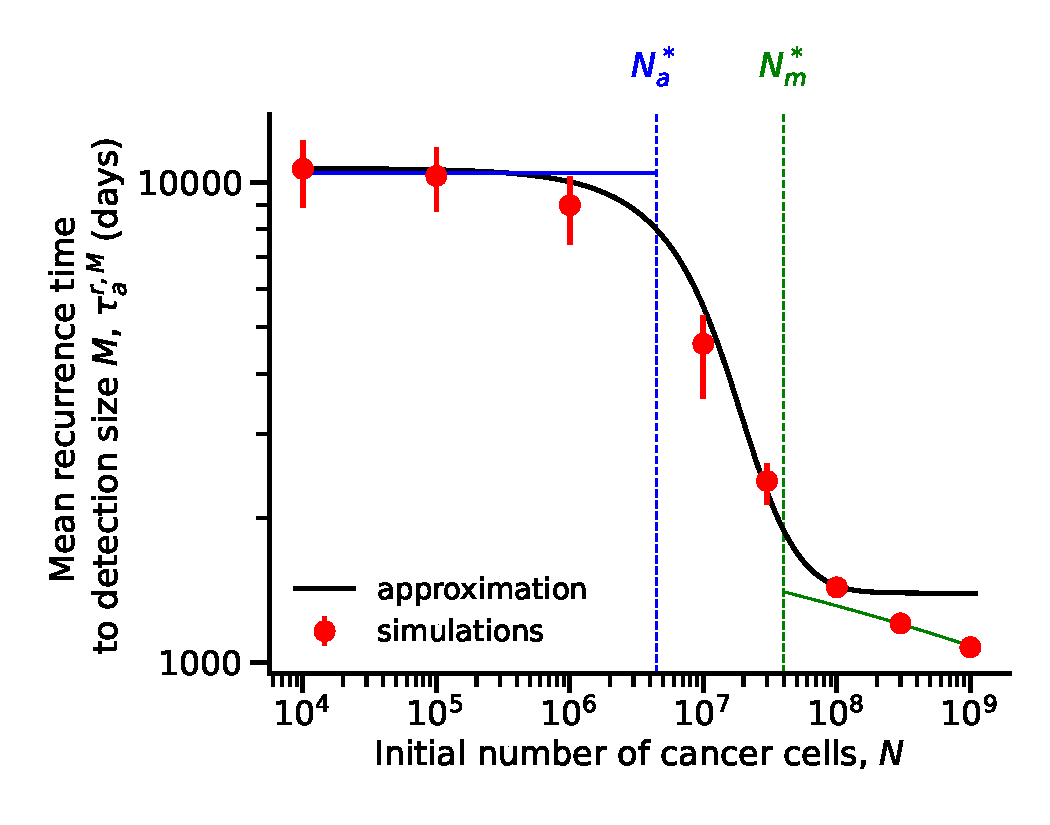
\includegraphics[width=1\textwidth]{Figures/RecurrencePlot.pdf}
\caption{The mean time for the mutant cell population to reach size $M$, where $M$ is the tumor detection size.
Our inhomogeneous Poisson-process approximation (solid black line, \cref{meanproliferationtime2}) is in agreement with simulation results (red markers with 95\% confidence intervals obtained with bootstrapping, see Appendix G) for small and intermediate values of $N$. Dashed vertical blue line represents the threshold tumor size above which evolutionary rescue is very likely through aneuploidy \cref{eq:N_a} and the dashed vertical green line represents the threshold tumor size above which evolutionary rescue is very likely through direct mutation \cref{eq:N_m}. Solid blue line represents the approximation \cref{meanproliferationtime2} with $\tau_a$ from \cref{eq:AsymptoticTimeRules} for $N<N_a^*$ and the solid green line  represents the approximation \cref{eq:t2det2} for $N>N_m^*$. The simulations converge to \cref{eq:t2det2} (green line) for large values of $N\gg N_m^*$.  Parameters: $\lambda_w=0.1,\lambda_a=0.0899,\lambda_m=0.1,\mu_w=0.14,\mu_a=0.09,\mu_m=0.09, u=10^{-2}, v=10^{-7}, M=10^7$.}
\label{RecurrencePlot}
\end{figure}
%%%
\begin{figure}
\vspace*{1\baselineskip}
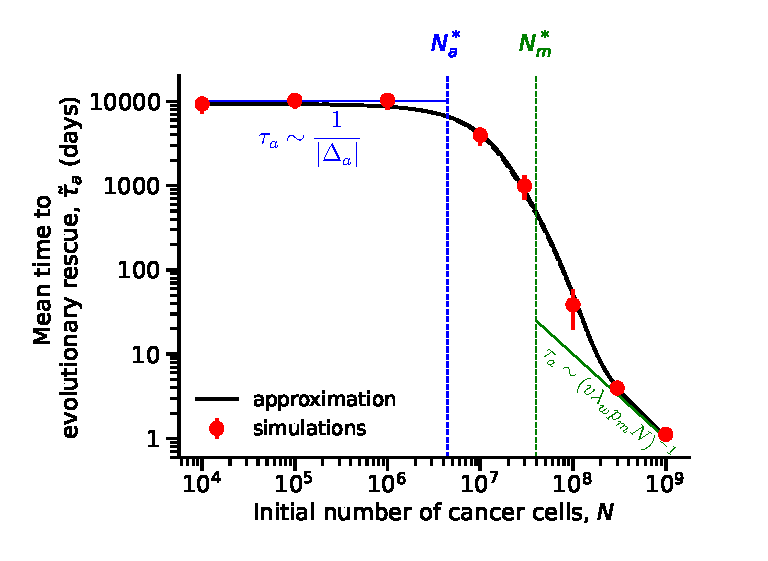
\includegraphics[width=1\textwidth]{Figures/SGVEvolutionaryRescueTimeComplete.pdf}
\caption{Shown is the mean time for appearance of a resistance mutation the leads to evolutionary rescue with aneuploidy ($u>0$). Black lines represent our inhomogeneous Poisson-process approximations (solid black line, \cref{meantimet2}; dashed black line \cref{meantimet2SGV}). Dashed black line is the  inhomogeneous Poisson-process approximation where a fraction $f$ of tumor is aneuploid at the onset of drug therapy which is in agreement with simulation results (red markers with 95\% confidence intervals obtained with bootstrapping, see Appendix G). Dashed vertical blue line represents the threshold tumor size above which evolutionary rescue is very likely through aneuploidy \cref{eq:N_a} and the dashed vertical green line represents the threshold tumor size above which evolutionary rescue is very likely through direct mutation \cref{eq:N_m}. Solid lines represents the approximations \cref{eq:AsymptoticTimeRules} ($N<N_a^*$ blue line and $N>N_m^*$ green line). 
Parameters: $\lambda_w=0.1,\lambda_m=0.0899,\lambda_m=0.1,\mu_w=0.14,\mu_a=0.09,\mu_m=0.09, u=10^{-2}, v=10^{-7},f=0.284\%$.}
\label{SGVEvolutionaryRescueTimeComplete}
\end{figure}
\end{appendices}
%%%%%%%%%%%%%%%%%%%%%%%%%%%%%%%%%%%%%%%%%%
\end{document}